% Capitolul 6: Modele VAR și Cauzalitate Granger
% Prezentare academică de calitate Harvard
% Program de licență, Academia de Studii Economice din București

\documentclass[9pt, aspectratio=169, t]{beamer}

% Asigură încadrarea conținutului pe diapozitive
\setbeamersize{text margin left=8mm, text margin right=8mm}

%=============================================================================
% CONFIGURARE TEMĂ ȘI STIL
%=============================================================================
\usetheme{Madrid}
\usecolortheme{seahorse}

% Paletă de Culori Profesională
\definecolor{MainBlue}{RGB}{26, 58, 110}
\definecolor{AccentBlue}{RGB}{42, 82, 140}
\definecolor{IDAred}{RGB}{220, 53, 69}
\definecolor{DarkGray}{RGB}{51, 51, 51}
\definecolor{MediumGray}{RGB}{128, 128, 128}
\definecolor{LightGray}{RGB}{248, 248, 248}
\definecolor{VeryLightGray}{RGB}{235, 235, 235}
\definecolor{Crimson}{RGB}{220, 53, 69}
\definecolor{Forest}{RGB}{46, 125, 50}
\definecolor{Amber}{RGB}{181, 133, 63}
\definecolor{Orange}{RGB}{230, 126, 34}
\definecolor{HarvardCrimson}{RGB}{165, 28, 48}

\setbeamercolor{palette primary}{bg=MainBlue, fg=white}
\setbeamercolor{palette secondary}{bg=MainBlue!85, fg=white}
\setbeamercolor{palette tertiary}{bg=MainBlue!70, fg=white}
\setbeamercolor{structure}{fg=MainBlue}
\setbeamercolor{title}{fg=MainBlue}
\setbeamercolor{frametitle}{fg=MainBlue, bg=white}
\setbeamercolor{block title}{bg=MainBlue, fg=white}
\setbeamercolor{block body}{bg=VeryLightGray, fg=DarkGray}
\setbeamercolor{block title alerted}{bg=Crimson, fg=white}
\setbeamercolor{block body alerted}{bg=Crimson!8, fg=DarkGray}
\setbeamercolor{block title example}{bg=Forest, fg=white}
\setbeamercolor{block body example}{bg=Forest!8, fg=DarkGray}
\setbeamercolor{item}{fg=MainBlue}

\setbeamertemplate{navigation symbols}{}

\setbeamertemplate{footline}{
    \leavevmode%
    \hbox{%
        \begin{beamercolorbox}[wd=.333333\paperwidth,ht=2.5ex,dp=1ex,center]{author in head/foot}%
            \usebeamerfont{author in head/foot}\insertshortauthor
        \end{beamercolorbox}%
        \begin{beamercolorbox}[wd=.333333\paperwidth,ht=2.5ex,dp=1ex,center]{title in head/foot}%
            \usebeamerfont{title in head/foot}\insertshorttitle
        \end{beamercolorbox}%
        \begin{beamercolorbox}[wd=.333333\paperwidth,ht=2.5ex,dp=1ex,right]{date in head/foot}%
            \usebeamerfont{date in head/foot}\insertshortdate{}\hspace*{2em}
            \insertframenumber{} / \inserttotalframenumber\hspace*{2ex}
        \end{beamercolorbox}}%
    \vskip0pt%
}

%=============================================================================
% PACHETE
%=============================================================================
\usepackage[utf8]{inputenc}
\usepackage[T1]{fontenc}
\usepackage{amsmath, amssymb, amsthm}
\usepackage{mathtools}
\usepackage{bm}
\usepackage{tikz}
\usetikzlibrary{arrows.meta, positioning, shapes, calc, decorations.pathreplacing}
\usepackage{booktabs}
\usepackage{multirow}
\usepackage{array}
\usepackage{graphicx}
\usepackage{hyperref}
\usepackage{colortbl}
\hypersetup{colorlinks=false, pdfborder={0 0 0}}
\graphicspath{{../logos/}{../charts/}}

%=============================================================================
% MEDII PENTRU TEOREME
%=============================================================================
\theoremstyle{definition}
\setbeamertemplate{theorems}[numbered]
\newtheorem{defn}{Definiție}
\newtheorem{thm}{Teoremă}
\newtheorem{prop}{Propoziție}
\newtheorem{rmk}{Observație}

%=============================================================================
% COMENZI PERSONALIZATE
%=============================================================================
\newcommand{\E}{\mathbb{E}}
\newcommand{\Var}{\text{Var}}
\newcommand{\Cov}{\text{Cov}}
\newcommand{\Corr}{\text{Corr}}
\newcommand{\R}{\mathbb{R}}
\newcommand{\N}{\mathbb{N}}
\newcommand{\Z}{\mathbb{Z}}
\newcommand{\RMSE}{\text{RMSE}}
\newcommand{\MAE}{\text{MAE}}
\newcommand{\MAPE}{\text{MAPE}}
\newcommand{\bY}{\mathbf{Y}}
\newcommand{\bX}{\mathbf{X}}
\newcommand{\bA}{\mathbf{A}}
\newcommand{\bB}{\mathbf{B}}
\newcommand{\bepsilon}{\boldsymbol{\varepsilon}}
\newcommand{\bSigma}{\boldsymbol{\Sigma}}

%=============================================================================
% INFORMAȚII TITLU
%=============================================================================
\title[Capitolul 6: VAR \& Granger]{Capitolul 6: Modele VAR și Cauzalitate Granger}
\subtitle{Program de licență, Facultatea de Cibernetică, Statistică și Informatică Economică, Academia de Studii Economice din București}
\author[Prof. dr. Daniel Traian Pele]{Prof. dr. Daniel Traian Pele\\[0.2cm]\footnotesize\texttt{danpele@ase.ro}}
\institute{Academia de Studii Economice din București}
\date{An Universitar 2025--2026}

\begin{document}

%=============================================================================
% DIAPOZITIV TITLU
%=============================================================================
\begin{frame}[plain]
    \begin{tikzpicture}[remember picture, overlay]
        \fill[IDAred] (current page.north west) rectangle ([yshift=-0.15cm]current page.north east);
        \node[anchor=north west] at ([xshift=0.5cm, yshift=-0.3cm]current page.north west) {
            \href{https://www.ase.ro}{\includegraphics[height=1.1cm]{ase_logo.png}}
        };
        \node[anchor=north] at ([yshift=-0.3cm]current page.north) {
            \href{https://ai4efin.ase.ro}{\includegraphics[height=1.1cm]{ai4efin_logo.png}}
        };
        \node[anchor=north east] at ([xshift=-0.5cm, yshift=-0.3cm]current page.north east) {
            \href{https://www.digital-finance-msca.com}{\includegraphics[height=1.1cm]{msca_logo.png}}
        };
    \end{tikzpicture}
    \vfill
    \begin{center}
        {\Large\textcolor{MediumGray}{Analiza și Prognoză Seriilor de Timp}}\\[0.3cm]
        {\Huge\textbf{\textcolor{MainBlue}{Capitolul 6: Modele VAR \& Cauzalitate Granger}}}\\[0.5cm]
        {\Large\textcolor{IDAred}{Serii de Timp Multivariate}}
    \end{center}
    \vfill

    \begin{tikzpicture}[remember picture, overlay]
        \fill[IDAred] (current page.south west) rectangle ([yshift=0.15cm]current page.south east);
        \node[anchor=south west] at ([xshift=0.5cm, yshift=0.8cm]current page.south west) {
            \href{https://theida.net}{\includegraphics[height=0.9cm]{ida_logo.png}}
        };
        \node[anchor=south] at ([xshift=-3cm, yshift=0.8cm]current page.south) {
            \href{https://blockchain-research-center.com}{\includegraphics[height=0.9cm]{brc_logo.png}}
        };
        \node[anchor=south] at ([yshift=0.8cm]current page.south) {
            \href{https://quantinar.com}{\includegraphics[height=0.9cm]{qr_logo.png}}
        };
        \node[anchor=south] at ([xshift=3cm, yshift=0.8cm]current page.south) {
            \href{https://quantlet.com}{\includegraphics[height=0.9cm]{ql_logo.png}}
        };
        \node[anchor=south east] at ([xshift=-0.5cm, yshift=0.8cm]current page.south east) {
            \href{https://ipe.ro/new}{\includegraphics[height=0.9cm]{acad_logo.png}}
        };
    \end{tikzpicture}
\end{frame}

%=============================================================================
% OUTLINE
%=============================================================================
\begin{frame}{Cuprins}
    \vspace{-0.3cm}
    {\small
    \begin{columns}[T]
        \begin{column}{0.48\textwidth}
            \tableofcontents[sections={1-5}, hideallsubsections]
        \end{column}
        \begin{column}{0.48\textwidth}
            \tableofcontents[sections={6-10}, hideallsubsections]
        \end{column}
    \end{columns}
    }
\end{frame}

%=============================================================================
% LEARNING OBJECTIVES
%=============================================================================
\begin{frame}{Obiective de Învățare}
    \begin{block}{La finalul acestui capitol, veți fi capabili să:}
        \begin{enumerate}
            \item Înțelegeți \textbf{motivația} pentru analiza multivariată a seriilor de timp
            \item Specificați și eștimați modele \textbf{VAR(p)}
            \item Aplicați teste de \textbf{cauzalitate Granger}
            \item Interpretați \textbf{funcțiile de răspuns la impuls (IRF)}
            \item Efectuați \textbf{descompunerea varianței erorii de prognoză (FEVD)}
            \item Selectați ordinul optimal al lag-urilor folosind criterii informaționale
            \item Implementați analiza VAR în \textbf{Python}
        \end{enumerate}
    \end{block}
\end{frame}

%=============================================================================
% MOTIVATION
%=============================================================================
\begin{frame}{Exemplu motivațional: Dinamică macroeconomică}
    \vspace{-0.3cm}
    \begin{center}
        \includegraphics[width=0.88\textwidth, height=0.62\textheight, keepaspectratio]{charts/ch5_motivation_econ.pdf}
    \end{center}
    \vspace{-0.2cm}
    {\footnotesize
    \begin{itemize}
        \item Variabilele economice sunt \textbf{interconectate}: PIB afectează șomajul, inflația afectează ratele dobânzilor
        \item Modificările unei variabile se \textbf{propagă} prin sistem
        \item Înțelegerea acestor dinamici necesită analiza \textbf{multivariată}
    \end{itemize}
    }
\end{frame}

\begin{frame}{Ideea cheie: Variabilele interacționează}
    \vspace{-0.3cm}
    \begin{center}
        \includegraphics[width=0.85\textwidth, height=0.60\textheight, keepaspectratio]{charts/ch5_motivation_scatter.pdf}
    \end{center}
    \vspace{-0.2cm}
    {\footnotesize
    \begin{itemize}
        \item \textbf{Legea lui Okun}: Creștere PIB mai mare $\Rightarrow$ șomaj mai mic
        \item \textbf{Regula Taylor}: Inflație mai mare $\Rightarrow$ rate ale dobânzii mai mari
        \item \textbf{Curba Phillips}: Compromis șomaj-inflație
    \end{itemize}
    }
\end{frame}

\begin{frame}{Relații de avans-întârziere}
    \vspace{-0.3cm}
    \begin{center}
        \includegraphics[width=0.88\textwidth, height=0.62\textheight, keepaspectratio]{charts/ch5_motivation_leadlag.pdf}
    \end{center}
    \vspace{-0.2cm}
    {\footnotesize
    \begin{itemize}
        \item Unele variabile \textbf{preced} altele: piața bursieră prezice activitatea economică
        \item Corelația încrucișată relevă \textbf{sincronizarea} relațiilor
        \item Corelație maximă la lag-ul 4: piața bursieră precede șomajul cu $\sim$4 luni
    \end{itemize}
    }
\end{frame}

\begin{frame}{De ce modelele univariate nu sunt suficiente}
    \vspace{-0.3cm}
    \begin{center}
        \includegraphics[width=0.92\textwidth, height=0.58\textheight, keepaspectratio]{charts/ch5_motivation_univariate.pdf}
    \end{center}
    \vspace{-0.2cm}
    {\footnotesize
    \begin{alertblock}{Problema}
        Modelele ARIMA tratează fiecare variabilă \textbf{izolat}---ignorând informații valoroase din alte variabile!
    \end{alertblock}
    \begin{exampleblock}{Soluția}
        \textbf{Modelele VAR} captează dinamică comună și efectele de feedback dîntre mai multe serii de timp.
    \end{exampleblock}
    }
\end{frame}

\begin{frame}{Ce vom învăța astăzi}
    \begin{block}{Concepte fundamentale}
        \begin{enumerate}
            \item \textbf{Modele VAR}: Cum să modelăm mai multe serii de timp împreună
            \item \textbf{Cauzalitate Granger}: Ajută $X$ la prezicerea lui $Y$?
            \item \textbf{Funcții de răspuns la impuls}: Cum se propagă șocurile?
            \item \textbf{Descompunerea varianței}: Ce determină fiecare variabilă?
        \end{enumerate}
    \end{block}

    \vspace{0.2cm}

    \begin{exampleblock}{Aplicații}
        \begin{itemize}
            \item Analiza politicii macroeconomice (efectele politicii monetare)
            \item Dinamică piețelor financiare (relații acțiuni-obligațiuni)
            \item Analiza ciclului de afaceri (indicători avansați)
            \item Managementul riscului (transmisia volatilității)
        \end{itemize}
    \end{exampleblock}
\end{frame}

%=============================================================================
% SECTION 1: INTRODUCTION
%=============================================================================
\section{Introducere în seriile de timp multivariate}

\begin{frame}{De ce analiza multivariată?}
    \begin{block}{Limitările modelelor univariate}
        \begin{itemize}
            \item Modelele ARIMA tratează fiecare variabilă \textbf{izolat}
            \item Ignoră potențialele \textbf{interacțiuni} între variabile
            \item Nu pot captura \textbf{efectele de feedback}
        \end{itemize}
    \end{block}

    \vspace{0.15cm}

    \begin{exampleblock}{Exemple economice de interdependență}
        \begin{itemize}
            \item PIB și șomaj (legea lui Okun)
            \item Rate ale dobânzii și inflație (regula Taylor)
            \item Prețuri acțiuni și volum tranzacționat
            \item Cursuri de schimb și balanță comercială
        \end{itemize}
    \end{exampleblock}
\end{frame}

\begin{frame}{Notația seriilor de timp multivariate}
    \begin{block}{Vector de variabile}
        Fie $\bY_t = (Y_{1t}, Y_{2t}, \ldots, Y_{Kt})'$ un vector $K \times 1$ de serii de timp.

        \vspace{0.2cm}
        Exemplu cu $K=2$:
        $$\bY_t = \begin{pmatrix} Y_{1t} \\ Y_{2t} \end{pmatrix} = \begin{pmatrix} \text{Creștere PIB}_t \\ \text{Inflație}_t \end{pmatrix}$$
    \end{block}

    \vspace{0.15cm}

    \begin{block}{Întrebări cheie}
        \begin{enumerate}
            \item Ajută $Y_1$ la prezicerea lui $Y_2$? (Cauzalitate Granger)
            \item Cum afectează șocurile în $Y_1$ pe $Y_2$? (Răspunsuri la impuls)
            \item Ce proporție din varianța lui $Y_2$ se datorează lui $Y_1$? (Descompunerea varianței)
        \end{enumerate}
    \end{block}
\end{frame}

\begin{frame}{Staționaritate multivariată}
    \begin{block}{Definiție: Staționaritate slabă}
        O serie de timp $K$-dimensională $\bY_t$ este \textbf{slab staționară} dacă:
        \begin{enumerate}
            \item $\E[\bY_t] = \boldsymbol{\mu}$ (vector de medie constant)
            \item $\Cov(\bY_t, \bY_{t-h}) = \boldsymbol{\Gamma}(h)$ depinde doar de $h$, nu de $t$
        \end{enumerate}
    \end{block}

    \vspace{0.15cm}

    \begin{block}{Matricea de autocovarianță}
        $$\boldsymbol{\Gamma}(h) = \E[(\bY_t - \boldsymbol{\mu})(\bY_{t-h} - \boldsymbol{\mu})'] = \begin{pmatrix} \gamma_{11}(h) & \gamma_{12}(h) \\ \gamma_{21}(h) & \gamma_{22}(h) \end{pmatrix}$$

        Notă: $\boldsymbol{\Gamma}(-h) = \boldsymbol{\Gamma}(h)'$ (transpusa, nu egală!)
    \end{block}
\end{frame}

\begin{frame}{Proprietăți ale covarianței încrucișate}
    {\small
    \hfill\begin{minipage}{0.9\textwidth}
    \begin{block}{Funcția de covarianță încrucișată}
        Pentru variabilele $Y_{it}$ și $Y_{jt}$:
        $$\gamma_{ij}(h) = \Cov(Y_{it}, Y_{j,t-h}) = \E[(Y_{it} - \mu_i)(Y_{j,t-h} - \mu_j)]$$
    \end{block}

    \begin{alertblock}{Diferența cheie față de cazul univariat}
        \begin{itemize}\setlength{\itemsep}{0pt}
            \item În general: $\gamma_{ij}(h) \neq \gamma_{ij}(-h)$
            \item Dar: $\gamma_{ij}(h) = \gamma_{ji}(-h)$
            \item Matricea de covarianță încrucișată \textbf{nu este simetrică} pentru $h \neq 0$
        \end{itemize}
    \end{alertblock}

    \begin{exampleblock}{Exemplu}
        Dacă $Y_1$ precede $Y_2$: $\gamma_{12}(h) > 0$ pentru $h > 0$ dar $\gamma_{12}(h) \approx 0$ pentru $h < 0$
    \end{exampleblock}
    \end{minipage}
    }
\end{frame}

\begin{frame}{Matricea funcției de corelație}
    \begin{block}{Definiție}
        \textbf{Matricea de autocorelație} la lag-ul $h$:
        $$\mathbf{R}(h) = \mathbf{D}^{-1} \boldsymbol{\Gamma}(h) \mathbf{D}^{-1}$$

        unde $\mathbf{D} = \text{diag}(\sigma_1, \sigma_2, \ldots, \sigma_K)$ și $\sigma_i = \sqrt{\gamma_{ii}(0)}$
    \end{block}

    \vspace{0.15cm}

    \begin{exampleblock}{Pentru cazul bivariat}
        $$\mathbf{R}(h) = \begin{pmatrix} \rho_{11}(h) & \rho_{12}(h) \\ \rho_{21}(h) & \rho_{22}(h) \end{pmatrix}$$

        unde $\rho_{ij}(h) = \frac{\gamma_{ij}(h)}{\sigma_i \sigma_j}$

        \vspace{0.2cm}
        Elementele diagonale: ACF obișnuite; Extra-diagonale: corelații încrucișate
    \end{exampleblock}
\end{frame}

%=============================================================================
% SECTION 2: VAR MODELS
%=============================================================================
\section{Vector Autoregresiv (VAR)}

\begin{frame}{Modelul VAR(p)}
    \begin{block}{Definiție}
        Un model \textbf{VAR(p)} pentru $K$ variabile:
        $$\bY_t = \mathbf{c} + \bA_1 \bY_{t-1} + \bA_2 \bY_{t-2} + \cdots + \bA_p \bY_{t-p} + \bepsilon_t$$

        unde:
        \begin{itemize}
            \item $\bY_t$: vector $K \times 1$ de variabile endogene
            \item $\mathbf{c}$: vector $K \times 1$ de constante
            \item $\bA_i$: matrice de coeficienți $K \times K$
            \item $\bepsilon_t$: vector $K \times 1$ de termeni de eroare cu $\E[\bepsilon_t] = \mathbf{0}$, $\E[\bepsilon_t \bepsilon_t'] = \bSigma$
        \end{itemize}
    \end{block}
\end{frame}

\begin{frame}{VAR(1) cu două variabile}
    \begin{block}{VAR(1) bivariat}
        $$\begin{pmatrix} Y_{1t} \\ Y_{2t} \end{pmatrix} = \begin{pmatrix} c_1 \\ c_2 \end{pmatrix} + \begin{pmatrix} a_{11} & a_{12} \\ a_{21} & a_{22} \end{pmatrix} \begin{pmatrix} Y_{1,t-1} \\ Y_{2,t-1} \end{pmatrix} + \begin{pmatrix} \varepsilon_{1t} \\ \varepsilon_{2t} \end{pmatrix}$$
    \end{block}

    \vspace{0.15cm}

    \begin{exampleblock}{Ecuație cu ecuație}
        \begin{align*}
            Y_{1t} &= c_1 + a_{11} Y_{1,t-1} + a_{12} Y_{2,t-1} + \varepsilon_{1t} \\
            Y_{2t} &= c_2 + a_{21} Y_{1,t-1} + a_{22} Y_{2,t-1} + \varepsilon_{2t}
        \end{align*}

        \textbf{Ideea cheie}: Fiecare ecuație include lag-uri ale \textbf{tuturor} variabilelor!
    \end{exampleblock}
\end{frame}

\begin{frame}{Exemplu numeric: VAR(1)}
    {\small
    \hfill\begin{minipage}{0.9\textwidth}
    \begin{exampleblock}{Model VAR(1) specific}
        $$\begin{pmatrix} Y_{1t} \\ Y_{2t} \end{pmatrix} = \begin{pmatrix} 0.5 \\ 0.3 \end{pmatrix} + \begin{pmatrix} 0.7 & 0.2 \\ -0.1 & 0.6 \end{pmatrix} \begin{pmatrix} Y_{1,t-1} \\ Y_{2,t-1} \end{pmatrix} + \begin{pmatrix} \varepsilon_{1t} \\ \varepsilon_{2t} \end{pmatrix}$$
    \end{exampleblock}

    \begin{block}{Interpretarea coeficienților}
        \begin{itemize}\setlength{\itemsep}{0pt}
            \item $a_{11} = 0.7$: O creștere de 1 unitate în $Y_1$ la $t-1$ crește $Y_1$ la $t$ cu 0.7
            \item $a_{12} = 0.2$: O creștere de 1 unitate în $Y_2$ la $t-1$ crește $Y_1$ la $t$ cu 0.2
            \item $a_{21} = -0.1$: O creștere de 1 unitate în $Y_1$ la $t-1$ \textbf{scade} $Y_2$ la $t$ cu 0.1
            \item $a_{22} = 0.6$: O creștere de 1 unitate în $Y_2$ la $t-1$ crește $Y_2$ la $t$ cu 0.6
        \end{itemize}
    \end{block}
    \end{minipage}
    }
\end{frame}

\begin{frame}{VAR(2): Dinamică de ordin superior}
    \begin{block}{Specificația VAR(2)}
        $$\bY_t = \mathbf{c} + \bA_1 \bY_{t-1} + \bA_2 \bY_{t-2} + \bepsilon_t$$

        Pentru $K=2$, modelul complet are $2 + 2 \times 4 + 2 \times 4 = 18$ parametri!
    \end{block}

    \vspace{0.15cm}

    \begin{exampleblock}{Dezvoltat}
        \begin{align*}
            Y_{1t} &= c_1 + a_{11}^{(1)} Y_{1,t-1} + a_{12}^{(1)} Y_{2,t-1} + a_{11}^{(2)} Y_{1,t-2} + a_{12}^{(2)} Y_{2,t-2} + \varepsilon_{1t} \\
            Y_{2t} &= c_2 + a_{21}^{(1)} Y_{1,t-1} + a_{22}^{(1)} Y_{2,t-1} + a_{21}^{(2)} Y_{1,t-2} + a_{22}^{(2)} Y_{2,t-2} + \varepsilon_{2t}
        \end{align*}
    \end{exampleblock}

    \vspace{0.15cm}

    {\footnotesize
    \begin{alertblock}{Blestemul dimensionalității}
        VAR($p$) cu $K$ variabile are $K + pK^2$ parametri. Cu $K=5$, $p=4$: $5 + 4 \times 25 = 105$ parametri!
    \end{alertblock}
    }
\end{frame}

\begin{frame}{Forma companion}
    \begin{block}{Conversia VAR(p) la VAR(1)}
        Orice VAR($p$) poate fi scris ca VAR(1) în \textbf{forma companion}:
        $$\boldsymbol{\xi}_t = \mathbf{A} \boldsymbol{\xi}_{t-1} + \mathbf{v}_t$$
    \end{block}

    \vspace{0.15cm}

    \begin{exampleblock}{Pentru VAR(2)}
        $$\underbrace{\begin{pmatrix} \bY_t \\ \bY_{t-1} \end{pmatrix}}_{\boldsymbol{\xi}_t} = \underbrace{\begin{pmatrix} \bA_1 & \bA_2 \\ \mathbf{I}_K & \mathbf{0} \end{pmatrix}}_{\mathbf{A}} \underbrace{\begin{pmatrix} \bY_{t-1} \\ \bY_{t-2} \end{pmatrix}}_{\boldsymbol{\xi}_{t-1}} + \underbrace{\begin{pmatrix} \bepsilon_t \\ \mathbf{0} \end{pmatrix}}_{\mathbf{v}_t}$$

        Matricea companion $\mathbf{A}$ este $Kp \times Kp$.
    \end{exampleblock}

    \vspace{0.15cm}

    {\footnotesize
    \begin{block}{De ce este utilă?}
        Staționaritatea, prognoză și IRF sunt mai ușor de analizat în forma companion.
    \end{block}
    }
\end{frame}

\begin{frame}{Proces VAR simulat}
    \vspace{-0.3cm}
    \begin{center}
        \includegraphics[width=0.82\textwidth, height=0.58\textheight, keepaspectratio]{charts/ch5_var_simulation.pdf}
    \end{center}
    \vspace{-0.2cm}
    {\footnotesize
    \begin{itemize}
        \item Două serii simulate dintr-un proces VAR(1) bivariat prezentând interdependența
        \item Fiecare variabilă răspunde atât la propriul trecut cât și la trecutul celeilalte variabile
        \item Observați cum seriile se mișcă împreună datorită dinamicii încrucișate
    \end{itemize}
    }
\end{frame}

\begin{frame}{Staționaritatea VAR}
    \begin{block}{Condiția de stabilitate}
        VAR(p) este \textbf{stabil} (staționar) dacă toate rădăcinile lui:
        $$\det(\mathbf{I}_K - \bA_1 z - \bA_2 z^2 - \cdots - \bA_p z^p) = 0$$
        se află \textbf{în afără} cercului unitate (adică $|z| > 1$).
    \end{block}

    \vspace{0.15cm}

    \begin{alertblock}{Pentru VAR(1)}
        Modelul este stabil dacă toate \textbf{valorile proprii} ale lui $\bA_1$ sunt mai mici decât 1 în valoare absolută.

        \vspace{0.2cm}
        Exemplu: Pentru $\bA_1 = \begin{pmatrix} 0.5 & 0.1 \\ 0.2 & 0.3 \end{pmatrix}$, valorile proprii sunt $\lambda_1 = 0.6$ și $\lambda_2 = 0.2$.

        Ambele $< 1$ $\Rightarrow$ stabil!
    \end{alertblock}
\end{frame}

\begin{frame}{Calculul valorilor proprii: Exemplu}
    {\small
    \hfill\begin{minipage}{0.9\textwidth}
    \begin{block}{Pentru $\bA = \begin{pmatrix} 0.7 & 0.2 \\ -0.1 & 0.6 \end{pmatrix}$}
        Polinomul caracteristic: $\det(\bA - \lambda \mathbf{I}) = 0$
        $$\det\begin{pmatrix} 0.7 - \lambda & 0.2 \\ -0.1 & 0.6 - \lambda \end{pmatrix} = (0.7-\lambda)(0.6-\lambda) + 0.02 = 0$$
        $$\lambda^2 - 1.3\lambda + 0.44 = 0$$
    \end{block}

    \begin{exampleblock}{Soluție}
        Folosind formula de gradul 2:
        $$\lambda = \frac{1.3 \pm \sqrt{1.69 - 1.76}}{2} = \frac{1.3 \pm \sqrt{-0.07}}{2} = 0.65 \pm 0.132i$$

        $|\lambda| = \sqrt{0.65^2 + 0.132^2} = \sqrt{0.44} = 0.663 < 1$ \quad $\checkmark$ Stabil!
    \end{exampleblock}
    \end{minipage}
    }
\end{frame}

\begin{frame}{Condiția de stabilitate: Interpretare vizuală}
    \vspace{-0.3cm}
    \begin{center}
        \includegraphics[width=0.82\textwidth, height=0.58\textheight, keepaspectratio]{charts/ch5_stability_roots.pdf}
    \end{center}
    \vspace{-0.2cm}
    {\footnotesize
    \begin{itemize}
        \item Valorile proprii ale matricei companion trebuie să fie în interiorul cercului unitate
        \item Valorile proprii complexe vin în perechi conjugate
        \item Dacă vreo valoare proprie este în afără cercului, VAR este exploziv (nestaționar)
    \end{itemize}
    }
\end{frame}

\begin{frame}{Media unui VAR staționar}
    \begin{block}{Media necondiționată}
        Pentru un VAR(1) staționar: $\bY_t = \mathbf{c} + \bA \bY_{t-1} + \bepsilon_t$

        Luând medii:
        $$\E[\bY_t] = \mathbf{c} + \bA \E[\bY_{t-1}]$$

        Deoarece $\E[\bY_t] = \E[\bY_{t-1}] = \boldsymbol{\mu}$ (staționaritate):
        $$\boldsymbol{\mu} = \mathbf{c} + \bA \boldsymbol{\mu} \quad \Rightarrow \quad \boldsymbol{\mu} = (\mathbf{I}_K - \bA)^{-1} \mathbf{c}$$
    \end{block}

    \vspace{0.15cm}

    \begin{exampleblock}{Exemplu}
        Dacă $\mathbf{c} = \begin{pmatrix} 0.5 \\ 0.3 \end{pmatrix}$ și $\bA = \begin{pmatrix} 0.7 & 0.2 \\ -0.1 & 0.6 \end{pmatrix}$:
        $$\boldsymbol{\mu} = \begin{pmatrix} 0.3 & -0.2 \\ 0.1 & 0.4 \end{pmatrix}^{-1} \begin{pmatrix} 0.5 \\ 0.3 \end{pmatrix} = \begin{pmatrix} 2.3 \\ 1.0 \end{pmatrix}$$
    \end{exampleblock}
\end{frame}

\begin{frame}{Structura covarianței pentru VAR(1)}
    {\small
    \hfill\begin{minipage}{0.9\textwidth}
    \begin{block}{Matricea varianță-covarianță $\boldsymbol{\Gamma}(0)$}
        Pentru VAR(1), varianța satisface \textbf{ecuația discretă Lyapunov}:
        $$\boldsymbol{\Gamma}(0) = \bA \boldsymbol{\Gamma}(0) \bA' + \bSigma$$
    \end{block}

    \begin{block}{Autocovarianța la lag-ul $h$}
        $$\boldsymbol{\Gamma}(h) = \bA^h \boldsymbol{\Gamma}(0), \quad h \geq 0$$

        Aceasta arată că autocovarianțele scad geometric cu valorile proprii ale lui $\bA$.
    \end{block}

    \begin{alertblock}{Rezolvarea ecuației Lyapunov}
        Se poate rezolvă prin vectorizare:
        $$\text{vec}(\boldsymbol{\Gamma}(0)) = (\mathbf{I}_{K^2} - \bA \otimes \bA)^{-1} \text{vec}(\bSigma)$$
        unde $\otimes$ denotă produsul Kronecker.
    \end{alertblock}
    \end{minipage}
    }
\end{frame}

\begin{frame}{Estimarea VAR}
    \begin{block}{Estimarea OLS}
        Fiecare ecuație poate fi eștimată prin \textbf{OLS separat}:
        $$\hat{\bA} = \left(\sum_{t=1}^{T} \bY_{t-1} \bY_{t-1}'\right)^{-1} \left(\sum_{t=1}^{T} \bY_{t-1} \bY_t'\right)$$

        \vspace{0.2cm}
        Aceasta este eficientă deoarece toate ecuațiile au \textbf{aceiași regresori}.
    \end{block}

    \vspace{0.15cm}

    \begin{block}{Matricea de covarianță}
        $$\hat{\bSigma} = \frac{1}{T-Kp-1} \sum_{t=1}^{T} \hat{\bepsilon}_t \hat{\bepsilon}_t'$$

        Erorile $\varepsilon_{1t}$ și $\varepsilon_{2t}$ pot fi \textbf{corelate contemporan}.
    \end{block}
\end{frame}

\begin{frame}{Selecția ordinului lag-ului}
    \begin{block}{Criterii informaționale}
        Alegem $p$ care minimizează:
        \begin{align*}
            \text{AIC}(p) &= \ln|\hat{\bSigma}_p| + \frac{2pK^2}{T} \\[0.2cm]
            \text{BIC}(p) &= \ln|\hat{\bSigma}_p| + \frac{pK^2 \ln T}{T} \\[0.2cm]
            \text{HQ}(p) &= \ln|\hat{\bSigma}_p| + \frac{2pK^2 \ln\ln T}{T}
        \end{align*}
    \end{block}

    \vspace{0.2cm}

    {\small
    \begin{block}{Îndrumări}
        \begin{itemize}
            \item AIC tinde să selecteze modele \textbf{mai mari} (mai bune pentru prognoză)
            \item BIC tinde să selecteze modele \textbf{mai mici} (selecție consistentă)
            \item Începeți cu $p_{max}$ maxim bazat pe frecvența datelor (ex. 4 pentru trimestrial, 12 pentru lunar)
        \end{itemize}
    \end{block}
    }
\end{frame}

\begin{frame}{Selecția lag-ului: Exemplu}
    \vspace{-0.3cm}
    \begin{center}
        \includegraphics[width=0.82\textwidth, height=0.58\textheight, keepaspectratio]{charts/ch5_lag_selection.pdf}
    \end{center}
    \vspace{-0.2cm}
    {\footnotesize
    \begin{itemize}
        \item Valorile criteriilor informaționale pentru diferite ordine ale lag-ului
        \item AIC și BIC pot sugera lag-uri optime diferite
        \item Valori mai mici indică o ajustare mai bună a modelului (penalizată de complexitate)
    \end{itemize}
    }
\end{frame}

\begin{frame}{Modele VAR restricționate}
    {\small
    \hfill\begin{minipage}{0.9\textwidth}
    \begin{block}{De ce restricționăm?}
        Modelele VAR complete pot fi \textbf{supraparametrizate}:
        \begin{itemize}\setlength{\itemsep}{0pt}
            \item Mulți coeficienți pot fi nesemnificativi
            \item Prognoze slabe
            \item Pierdere de grade de libertate
        \end{itemize}
    \end{block}

    \begin{block}{Restricții comune}
        \begin{itemize}\setlength{\itemsep}{0pt}
            \item \textbf{Restricții de zero}: Setăm coeficienți mici la zero
            \item \textbf{Exogenitate de bloc}: Unele variabile nu afectează altele
            \item \textbf{Excluderea lag-urilor}: Excludem anumite lag-uri
        \end{itemize}
    \end{block}

    \begin{alertblock}{Testarea restricțiilor}
        Folosim testul raportului de verosimilitate:
        $LR = T(\ln|\hat{\bSigma}_R| - \ln|\hat{\bSigma}_U|) \sim \chi^2_r$

        unde $r$ = numărul de restricții
    \end{alertblock}
    \end{minipage}
    }
\end{frame}

%=============================================================================
% SECTION 3: GRANGER CAUSALITY
%=============================================================================
\section{Cauzalitate Granger}

\begin{frame}{Ce este cauzalitatea Granger?}
    \begin{block}{Clive Granger (1969, Premiul Nobel 2003)}
        ``$X$ \textbf{cauzează Granger} pe $Y$'' dacă valorile trecute ale lui $X$ ajută la prezicerea lui $Y$, \textbf{dincolo de} ce pot prezice valorile trecute ale lui $Y$ singure.
    \end{block}

    \vspace{0.15cm}

    \begin{alertblock}{Distincție importantă}
        \textbf{Cauzalitate Granger $\neq$ Cauzalitate reală}

        \begin{itemize}
            \item Cauzalitatea Granger este despre \textbf{conținut predictiv}
            \item NU implică cauzare economică/structurală
            \item ``$X$ cauzează Granger pe $Y$'' înseamnă: $X$ conține informații utile pentru prognoză lui $Y$
        \end{itemize}
    \end{alertblock}
\end{frame}

\begin{frame}{Definiție formală}
    \begin{block}{Cauzalitate Granger}
        $X$ \textbf{nu cauzează Granger} pe $Y$ dacă:
        $$\E[Y_t | Y_{t-1}, Y_{t-2}, \ldots, X_{t-1}, X_{t-2}, \ldots] = \E[Y_t | Y_{t-1}, Y_{t-2}, \ldots]$$

        Cu alte cuvinte: adăugarea istoricului lui $X$ nu îmbunătățește predicția lui $Y$.
    \end{block}

    \vspace{0.15cm}

    \begin{exampleblock}{În contextul VAR}
        Pentru VAR(1): $Y_{1t} = c_1 + a_{11} Y_{1,t-1} + a_{12} Y_{2,t-1} + \varepsilon_{1t}$

        \vspace{0.2cm}
        $Y_2$ \textbf{nu} cauzează Granger pe $Y_1$ dacă $a_{12} = 0$.

        \vspace{0.2cm}
        Pentru VAR(p): $Y_2$ nu cauzează Granger pe $Y_1$ dacă $a_{12}^{(1)} = a_{12}^{(2)} = \cdots = a_{12}^{(p)} = 0$.
    \end{exampleblock}
\end{frame}

\begin{frame}{Testarea cauzalității Granger}
    \begin{block}{Ipotezele testului}
        \textbf{$H_0$}: $Y_2$ \textbf{nu} cauzează Granger pe $Y_1$

        $$H_0: a_{12}^{(1)} = a_{12}^{(2)} = \cdots = a_{12}^{(p)} = 0$$

        \textbf{$H_1$}: Cel puțin un $a_{12}^{(i)} \neq 0$ (există cauzalitate Granger)
    \end{block}

    \vspace{0.15cm}

    \begin{block}{Statistica testului: Testul Wald}
        $$F = \frac{(RSS_R - RSS_U)/p}{RSS_U/(T-2p-1)} \sim F_{p, T-2p-1}$$

        unde:
        \begin{itemize}
            \item $RSS_R$: Suma pătratelor reziduurilor din modelul restricționat (fără lag-urile lui $Y_2$)
            \item $RSS_U$: Suma pătratelor reziduurilor din modelul nerestricționat (VAR complet)
        \end{itemize}
    \end{block}
\end{frame}

\begin{frame}{Tipuri de cauzalitate Granger}
    \begin{center}
    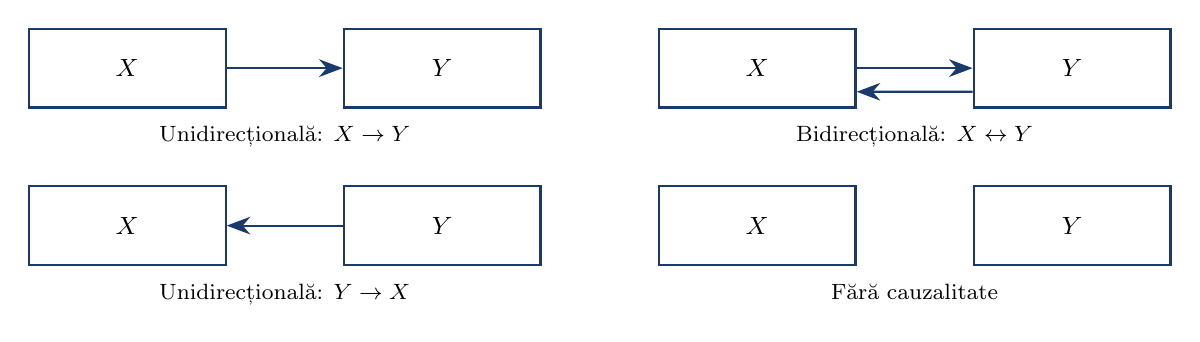
\begin{tikzpicture}[
        box/.style={rectangle, draw=MainBlue, thick, minimum width=2.5cm, minimum height=1cm, font=\small},
        arrow/.style={-{Stealth[length=3mm]}, thick, MainBlue}
    ]
        % Unidirectional X -> Y
        \node[box] (x1) at (0, 2) {$X$};
        \node[box] (y1) at (4, 2) {$Y$};
        \draw[arrow] (x1) -- (y1);
        \node[below=0.1cm of x1, xshift=2cm, font=\footnotesize] {Unidirecțională: $X \rightarrow Y$};

        % Unidirectional Y -> X
        \node[box] (x2) at (0, 0) {$X$};
        \node[box] (y2) at (4, 0) {$Y$};
        \draw[arrow] (y2) -- (x2);
        \node[below=0.1cm of x2, xshift=2cm, font=\footnotesize] {Unidirecțională: $Y \rightarrow X$};

        % Bidirectional
        \node[box] (x3) at (8, 2) {$X$};
        \node[box] (y3) at (12, 2) {$Y$};
        \draw[arrow] (x3.east) -- (y3.west);
        \draw[arrow] (y3.west) ++(0, -0.3) -- (x3.east |- {0, 1.7});
        \node[below=0.1cm of x3, xshift=2cm, font=\footnotesize] {Bidirecțională: $X \leftrightarrow Y$};

        % No causality
        \node[box] (x4) at (8, 0) {$X$};
        \node[box] (y4) at (12, 0) {$Y$};
        \node[below=0.1cm of x4, xshift=2cm, font=\footnotesize] {Fără cauzalitate};
    \end{tikzpicture}
    \end{center}

    \vspace{0.15cm}

    {\small
    \begin{block}{Exemple economice}
        \begin{itemize}
            \item Masa monetară $\rightarrow$ Producție? (viziunea monetaristă)
            \item Prețurile acțiunilor $\leftrightarrow$ Volumul tranzacționat (bidirecțională)
            \item Vremea $\rightarrow$ Recolta (unidirecțională, evident)
        \end{itemize}
    \end{block}
    }
\end{frame}

\begin{frame}{Funcția de corelație încrucișată}
    {\small
    \hfill\begin{minipage}{0.9\textwidth}
    \begin{defn}[Funcția de corelație încrucișată]
        \textbf{Corelația încrucișată} între $X_t$ și $Y_t$ la lag-ul $k$ este:
        $$\rho_{XY}(k) = \frac{\gamma_{XY}(k)}{\sigma_X \sigma_Y} = \frac{\Cov(X_t, Y_{t+k})}{\sqrt{\Var(X_t)\Var(Y_t)}}$$
    \end{defn}

    \begin{block}{Interpretare}
        \begin{itemize}\setlength{\itemsep}{0pt}
            \item $\rho_{XY}(k) > 0$ la $k > 0$: $X$ este corelat pozitiv cu $Y$ viitor (X poate precede Y)
            \item $\rho_{XY}(k) > 0$ la $k < 0$: $X$ este corelat pozitiv cu $Y$ trecut (Y poate precede X)
        \end{itemize}
    \end{block}

    \begin{alertblock}{Notă}
        Spre deosebire de ACF, corelația încrucișată \textbf{nu este simetrică}: $\rho_{XY}(k) \neq \rho_{XY}(-k)$ în general.
    \end{alertblock}
    \end{minipage}
    }
\end{frame}

\begin{frame}{Corelație încrucișată: Ilustrare vizuală}
    \begin{center}
        \includegraphics[width=0.95\textwidth]{charts/ch5_def_ccf.pdf}
    \end{center}
    \vspace{-0.2cm}
    \small Stânga: două serii înrudite. Dreapta: CCF relevă că $X$ precede $Y$ (corelații semnificative la lag-uri pozitive).
\end{frame}

\begin{frame}{Cauzalitate Granger: Considerații practice}
    \begin{alertblock}{Capcane comune}
        \begin{enumerate}
            \item \textbf{Variabile omise}: O a treia variabilă $Z$ poate cauza atât $X$ cât și $Y$
            \item \textbf{Nestaționaritate}: Testul necesită date staționare (sau cointegrare)
            \item \textbf{Selecția lag-ului}: Rezultatele pot fi sensibile la $p$
            \item \textbf{Mărimea eșantionului}: Necesită suficiente observații
        \end{enumerate}
    \end{alertblock}

    \vspace{0.15cm}

    \begin{block}{Bune practici}
        \begin{itemize}
            \item Testați mai întâi pentru rădăcini unitare
            \item Folosiți criterii multiple pentru selecția lag-ului
            \item Verificați robustețea la diferite ordine ale lag-ului
            \item Raportați rezultatele pentru ambele direcții
        \end{itemize}
    \end{block}
\end{frame}

\begin{frame}{Test cauzalitate Granger: Exemplu numeric}
    {\small
    \hfill\begin{minipage}{0.9\textwidth}
    \begin{exampleblock}{Testare: Cauzează creșterea masei monetare Granger producția?}
        \textbf{Model nerestricționat} (VAR cu 2 lag-uri):
        $$\Delta Y_t = c + \alpha_1 \Delta Y_{t-1} + \alpha_2 \Delta Y_{t-2} + \beta_1 \Delta M_{t-1} + \beta_2 \Delta M_{t-2} + \varepsilon_t$$

        \textbf{Model restricționat} ($H_0$: $\beta_1 = \beta_2 = 0$):
        $$\Delta Y_t = c + \alpha_1 \Delta Y_{t-1} + \alpha_2 \Delta Y_{t-2} + \varepsilon_t$$
    \end{exampleblock}

    \begin{block}{Calculul testului}
        Cu $T = 100$, $RSS_U = 45.2$, $RSS_R = 52.8$:
        $$F = \frac{(52.8 - 45.2)/2}{45.2/(100 - 5)} = \frac{3.8}{0.476} = 7.98$$

        $F_{0.05}(2, 95) = 3.09$ $\Rightarrow$ \textbf{Respingem $H_0$}: Banii cauzează Granger producția!
    \end{block}
    \end{minipage}
    }
\end{frame}

\begin{frame}{Procedura Toda-Yamamoto}
    {\small
    \hfill\begin{minipage}{0.9\textwidth}
    \begin{alertblock}{Problema cu datele nestaționare}
        Testul Granger standard are \textbf{distribuții non-standard} când:
        \begin{itemize}\setlength{\itemsep}{0pt}
            \item Variabilele au rădăcini unitare
            \item Variabilele sunt cointegrate
        \end{itemize}
    \end{alertblock}

    \begin{block}{Soluția Toda-Yamamoto (1995)}
        \begin{enumerate}\setlength{\itemsep}{0pt}
            \item Determinăm ordinul maxim de integrare $d_{max}$
            \item Eștimăm VAR($p + d_{max}$) în \textbf{niveluri}
            \item Testăm restricții doar pe primele $p$ lag-uri
            \item Lag-urile suplimentare $d_{max}$ \textbf{nu sunt} testate (doar pentru distribuția corectă)
        \end{enumerate}
    \end{block}

    \begin{exampleblock}{Avantaj}
        Testul Wald are distribuție asimptotică $\chi^2$ indiferent de cointegrare!
    \end{exampleblock}
    \end{minipage}
    }
\end{frame}

\begin{frame}{Cauzalitate instantanee}
    \begin{block}{Definiție}
        $X$ \textbf{cauzează instantaneu} pe $Y$ dacă:
        $$\E[Y_t | \Omega_{t-1}, X_t] \neq \E[Y_t | \Omega_{t-1}]$$

        unde $\Omega_{t-1}$ conține toate informațiile trecute.
    \end{block}

    \vspace{0.15cm}

    \begin{block}{Testarea în VAR}
        Testăm dacă $\sigma_{12} \neq 0$ în matricea de covarianță:
        $$\bSigma = \begin{pmatrix} \sigma_1^2 & \sigma_{12} \\ \sigma_{12} & \sigma_2^2 \end{pmatrix}$$

        Dacă $\sigma_{12} = 0$: nu există cauzalitate instantanee
    \end{block}

    \vspace{0.15cm}

    {\footnotesize
    \begin{alertblock}{Interpretare}
        Cauzalitatea instantanee reflectă adesea \textbf{șocuri comune} sau \textbf{agregarea datelor}, nu efecte contemporane reale.
    \end{alertblock}
    }
\end{frame}

\begin{frame}{Cauzalitate Granger în sisteme multiple}
    \begin{block}{Testul exogenității de bloc}
        Într-un VAR cu $K > 2$ variabile, testăm dacă un \textbf{grup} de variabile cauzează Granger un alt grup.

        \vspace{0.2cm}
        Exemplu: Cauzează variabilele financiare (rate ale dobânzii, prețuri acțiuni) Granger variabilele reale (PIB, șomaj)?
    \end{block}

    \vspace{0.15cm}

    \begin{exampleblock}{Statistica testului}
        $$\chi^2 = T \cdot K_1 \cdot p \cdot \left(\ln|\hat{\bSigma}_R| - \ln|\hat{\bSigma}_U|\right) \sim \chi^2_{K_1 \cdot K_2 \cdot p}$$

        unde $K_1$ = numărul de variabile ``cauzate'', $K_2$ = numărul de variabile ``cauzatoare''
    \end{exampleblock}
\end{frame}

%=============================================================================
% SECTION 4: IMPULSE RESPONSE FUNCTIONS
%=============================================================================
\section{Funcții de răspuns la impuls}

\begin{frame}{Ce sunt funcțiile de răspuns la impuls?}
    \begin{block}{Definiție}
        O \textbf{Funcție de Răspuns la Impuls (IRF)} trasează efectul unui șoc punctual la o variabilă asupra valorilor curente și viitoare ale tuturor variabilelor.
    \end{block}

    \vspace{0.15cm}

    \begin{exampleblock}{Întrebarea la care răspund IRF-urile}
        ``Dacă există un șoc neașteptat de 1 unitate la $Y_1$ astăzi, ce se întâmplă cu $Y_1$ și $Y_2$ în următoarele $h$ perioade?''
    \end{exampleblock}

    \vspace{0.15cm}

    \begin{block}{Reprezentarea MA($\infty$)}
        Un VAR(p) stabil poate fi scris ca:
        $$\bY_t = \boldsymbol{\mu} + \sum_{i=0}^{\infty} \boldsymbol{\Phi}_i \bepsilon_{t-i}$$

        Matricele $\boldsymbol{\Phi}_i$ sunt \textbf{răspunsurile la impuls} la orizontul $i$.
    \end{block}
\end{frame}

\begin{frame}{Calculul IRF pentru VAR(1)}
    \begin{block}{Pentru VAR(1): $\bY_t = \mathbf{c} + \bA \bY_{t-1} + \bepsilon_t$}
        Matricele de răspuns la impuls sunt:
        $$\boldsymbol{\Phi}_0 = \mathbf{I}_K, \quad \boldsymbol{\Phi}_1 = \bA, \quad \boldsymbol{\Phi}_2 = \bA^2, \quad \ldots, \quad \boldsymbol{\Phi}_h = \bA^h$$
    \end{block}

    \vspace{0.15cm}

    \begin{exampleblock}{Interpretare}
        $[\boldsymbol{\Phi}_h]_{ij}$ = Efectul asupra lui $Y_i$ la momentul $t+h$ al unui șoc unitar la $Y_j$ la momentul $t$

        \vspace{0.2cm}
        Pentru VAR stabil: $\boldsymbol{\Phi}_h \rightarrow \mathbf{0}$ când $h \rightarrow \infty$ (șocurile dispar)
    \end{exampleblock}
\end{frame}

\begin{frame}{Calculul IRF pentru VAR(p) general}
    {\small
    \hfill\begin{minipage}{0.9\textwidth}
    \begin{block}{Formula recursivă pentru VAR(p)}
        Pentru $\bY_t = \mathbf{c} + \bA_1\bY_{t-1} + \bA_2\bY_{t-2} + \cdots + \bA_p\bY_{t-p} + \bepsilon_t$:
        $$\boldsymbol{\Phi}_h = \sum_{j=1}^{\min(h,p)} \bA_j \boldsymbol{\Phi}_{h-j}, \quad h = 1, 2, 3, \ldots$$
        cu $\boldsymbol{\Phi}_0 = \mathbf{I}_K$ și $\boldsymbol{\Phi}_h = \mathbf{0}$ pentru $h < 0$.
    \end{block}

    \begin{exampleblock}{Exemplu: IRF pentru VAR(2)}
        \begin{itemize}\setlength{\itemsep}{0pt}
            \item $\boldsymbol{\Phi}_0 = \mathbf{I}_K$
            \item $\boldsymbol{\Phi}_1 = \bA_1 \boldsymbol{\Phi}_0 = \bA_1$
            \item $\boldsymbol{\Phi}_2 = \bA_1 \boldsymbol{\Phi}_1 + \bA_2 \boldsymbol{\Phi}_0 = \bA_1^2 + \bA_2$
            \item $\boldsymbol{\Phi}_3 = \bA_1 \boldsymbol{\Phi}_2 + \bA_2 \boldsymbol{\Phi}_1 = \bA_1(\bA_1^2 + \bA_2) + \bA_2\bA_1$
        \end{itemize}
    \end{exampleblock}
    \end{minipage}
    }
\end{frame}

\begin{frame}{IRF ortogonalizate}
    \begin{alertblock}{Problema: Erori corelate}
        Dacă $\bSigma$ nu este diagonală, șocurile $\varepsilon_{1t}$ și $\varepsilon_{2t}$ sunt corelate.

        Un șoc la ``$Y_1$'' implică și un șoc la ``$Y_2$''.
    \end{alertblock}

    \vspace{0.15cm}

    \begin{block}{Soluție: Descompunerea Cholesky}
        Factorizăm $\bSigma = \mathbf{P}\mathbf{P}'$ unde $\mathbf{P}$ este inferior triunghiulară.

        Definim șocuri ortogonalizate: $\mathbf{u}_t = \mathbf{P}^{-1}\bepsilon_t$ cu $\E[\mathbf{u}_t \mathbf{u}_t'] = \mathbf{I}$

        \vspace{0.2cm}
        IRF ortogonalizate: $\boldsymbol{\Theta}_h = \boldsymbol{\Phi}_h \mathbf{P}$
    \end{block}

    \vspace{0.2cm}

    {\small
    \begin{alertblock}{Ordinea contează!}
        Cholesky presupune variabilele ordonate de la ``cea mai exogenă'' la ``cea mai endogenă''. Rezultatele depind de această ordine.
    \end{alertblock}
    }
\end{frame}

\begin{frame}{Funcții de răspuns la impuls: Exemplu}
    \vspace{-0.3cm}
    \begin{center}
        \includegraphics[width=0.82\textwidth, height=0.58\textheight, keepaspectratio]{charts/ch5_irf.pdf}
    \end{center}
    \vspace{-0.2cm}
    {\footnotesize
    \begin{itemize}
        \item IRF arată cum răspunde fiecare variabilă la un șoc unitar în timp
        \item Zonele umbrite reprezintă intervale de încredere (incertitudine în eștimări)
        \item Pentru modele VAR stabile, răspunsurile converg la zero pe măsură ce orizontul crește
    \end{itemize}
    }
\end{frame}

\begin{frame}{Exemplu numeric IRF}
    {\small
    \hfill\begin{minipage}{0.9\textwidth}
    \begin{block}{Pentru $\bA = \begin{pmatrix} 0.7 & 0.2 \\ -0.1 & 0.6 \end{pmatrix}$}
        \begin{align*}
            \boldsymbol{\Phi}_0 &= \begin{pmatrix} 1 & 0 \\ 0 & 1 \end{pmatrix} \\
            \boldsymbol{\Phi}_1 &= \bA = \begin{pmatrix} 0.7 & 0.2 \\ -0.1 & 0.6 \end{pmatrix} \\
            \boldsymbol{\Phi}_2 &= \bA^2 = \begin{pmatrix} 0.47 & 0.26 \\ -0.13 & 0.34 \end{pmatrix}
        \end{align*}
    \end{block}

    \begin{exampleblock}{Interpretare}
        \begin{itemize}\setlength{\itemsep}{0pt}
            \item $[\boldsymbol{\Phi}_2]_{12} = 0.26$: Un șoc unitar la $Y_2$ crește $Y_1$ cu 0.26 după 2 perioade
            \item $[\boldsymbol{\Phi}_2]_{21} = -0.13$: Un șoc unitar la $Y_1$ \textbf{scade} $Y_2$ cu 0.13 după 2 perioade
        \end{itemize}
    \end{exampleblock}
    \end{minipage}
    }
\end{frame}

\begin{frame}{Răspunsuri la impuls cumulative}
    \begin{block}{Definiție}
        \textbf{IRF cumulativ} până la orizontul $H$:
        $$\boldsymbol{\Psi}_H = \sum_{h=0}^{H} \boldsymbol{\Phi}_h$$

        Măsoară \textbf{efectul total acumulat} al unui șoc.
    \end{block}

    \vspace{0.15cm}

    \begin{exampleblock}{Multiplicatorul pe termen lung}
        Pentru VAR stabil: $\boldsymbol{\Psi}_\infty = (\mathbf{I}_K - \bA_1 - \bA_2 - \cdots - \bA_p)^{-1}$

        \vspace{0.2cm}
        Aceasta dă \textbf{efectul permanent} al unui șoc punctual.
    \end{exampleblock}

    \vspace{0.15cm}

    {\footnotesize
    \begin{alertblock}{Când să folosim}
        IRF cumulative sunt utile când ne interesează impactul total (ex. pierderea cumulată de PIB după un șoc).
    \end{alertblock}
    }
\end{frame}

\begin{frame}{Intervale de încredere pentru IRF}
    {\small
    \hfill\begin{minipage}{0.9\textwidth}
    \begin{block}{Surse de incertitudine}
        IRF sunt funcții de parametrii eștimați $\hat{\bA}_1, \ldots, \hat{\bA}_p$, deci au \textbf{incertitudine de eșantionare}.
    \end{block}

    \begin{block}{Metode pentru benzi de încredere}
        \begin{enumerate}\setlength{\itemsep}{0pt}
            \item \textbf{Asimptotice}: Folosim metoda delta pentru a deriva erorile standard
            \item \textbf{Monte Carlo}: Simulăm din distribuția asimptotică a lui $\hat{\bA}$
            \item \textbf{Bootstrap}: Reeșantionăm reziduurile și reeștimăm VAR
        \end{enumerate}
    \end{block}

    \begin{alertblock}{Procedura Bootstrap}
        \begin{enumerate}\setlength{\itemsep}{0pt}
            \item Eștimăm VAR, salvăm reziduurile $\{\hat{\bepsilon}_t\}$
            \item Extragem cu înlocuire pentru a crea $\{\hat{\bepsilon}_t^*\}$
            \item Generăm eșantion bootstrap folosind VAR eștimat
            \item Reeștimăm și calculăm IRF
            \item Repetăm de $B$ ori; folosim percentilele pentru IC
        \end{enumerate}
    \end{alertblock}
    \end{minipage}
    }
\end{frame}

\begin{frame}{VAR Structural (SVAR)}
    \begin{block}{Motivație}
        Șocurile VAR standard $\bepsilon_t$ sunt inovații de \textbf{formă redusă}---combinații liniare de șocuri structurale.

        \vspace{0.2cm}
        Vrem să identificăm \textbf{șocuri structurale} semnificative economic.
    \end{block}

    \vspace{0.15cm}

    \begin{block}{Forma structurală}
        $$\mathbf{B}_0 \bY_t = \boldsymbol{\Gamma}_0 + \mathbf{B}_1 \bY_{t-1} + \cdots + \mathbf{B}_p \bY_{t-p} + \mathbf{u}_t$$

        unde $\mathbf{u}_t$ sunt \textbf{șocuri structurale} cu $\E[\mathbf{u}_t \mathbf{u}_t'] = \mathbf{I}_K$
    \end{block}

    \vspace{0.15cm}

    {\footnotesize
    \begin{exampleblock}{Relația cu forma redusă}
        $\bepsilon_t = \mathbf{B}_0^{-1} \mathbf{u}_t \quad \Rightarrow \quad \bSigma = \mathbf{B}_0^{-1} (\mathbf{B}_0^{-1})'$
    \end{exampleblock}
    }
\end{frame}

\begin{frame}{Identificare în SVAR}
    {\small
    \hfill\begin{minipage}{0.9\textwidth}
    \begin{alertblock}{Problema identificării}
        $\bSigma$ are $K(K+1)/2$ elemente unice, dar $\mathbf{B}_0^{-1}$ are $K^2$ elemente.

        \vspace{0.2cm}
        Avem nevoie de $K(K-1)/2$ restricții suplimentare!
    \end{alertblock}

    \begin{block}{Scheme comune de identificare}
        \begin{enumerate}\setlength{\itemsep}{0pt}
            \item \textbf{Restricții pe termen scurt}: Efecte de impact zero (Cholesky)
            \item \textbf{Restricții pe termen lung}: Efecte zero pe termen lung (Blanchard-Quah)
            \item \textbf{Restricții de semn}: Constrângeri de inegalitate pe IRF
            \item \textbf{Instrumente externe}: Folosim informații din afară
        \end{enumerate}
    \end{block}

    \begin{exampleblock}{Exemplu: Ordonare Cholesky (recursivă)}
        Pentru $K=2$: $\mathbf{B}_0^{-1} = \begin{pmatrix} b_{11} & 0 \\ b_{21} & b_{22} \end{pmatrix}$

        Variabila 1 nu răspunde la șocul 2 contemporan.
    \end{exampleblock}
    \end{minipage}
    }
\end{frame}

\begin{frame}{Exemplu IRF structural}
    \vspace{-0.3cm}
    \begin{center}
        \includegraphics[width=0.82\textwidth, height=0.58\textheight, keepaspectratio]{charts/ch5_structural_irf.pdf}
    \end{center}
    \vspace{-0.2cm}
    {\footnotesize
    \begin{itemize}
        \item IRF structurale bazate pe identificare Cholesky
        \item Ordinea variabilelor afectează interpretarea șocurilor
        \item Prima variabilă răspunde doar la propriile șocuri contemporan
    \end{itemize}
    }
\end{frame}

%=============================================================================
% SECTION 5: FORECAST ERROR VARIANCE DECOMPOSITION
%=============================================================================
\section{Descompunerea varianței erorii de prognoză}

\begin{frame}{Descompunerea varianței}
    \begin{alertblock}{Întrebare}
        Ce proporție din varianța erorii de prognoză a lui $Y_i$ la orizontul $h$ se datorează șocurilor la $Y_j$?
    \end{alertblock}

    \vspace{0.15cm}

    \begin{block}{Formula FEVD}
        $$\text{FEVD}_{ij}(h) = \frac{\sum_{s=0}^{h-1} [\boldsymbol{\Theta}_s]_{ij}^2}{\sum_{s=0}^{h-1} \sum_{k=1}^{K} [\boldsymbol{\Theta}_s]_{ik}^2}$$

        \vspace{0.2cm}
        Aceasta dă \textbf{procentul} din varianța prognozei la $h$ pași a lui $Y_i$ explicat de șocurile la $Y_j$.
    \end{block}

    \vspace{0.2cm}

    {\small
    \begin{exampleblock}{Proprietăți}
        \begin{itemize}
            \item $0 \leq \text{FEVD}_{ij}(h) \leq 1$
            \item $\sum_{j=1}^{K} \text{FEVD}_{ij}(h) = 1$ (suma la 100\%)
            \item La $h=1$: Șocurile proprii domină (prin construcția Cholesky)
        \end{itemize}
    \end{exampleblock}
    }
\end{frame}

\begin{frame}{FEVD: Exemplu}
    \vspace{-0.3cm}
    \begin{center}
        \includegraphics[width=0.82\textwidth, height=0.58\textheight, keepaspectratio]{charts/ch5_fevd.pdf}
    \end{center}
    \vspace{-0.2cm}
    {\footnotesize
    \begin{itemize}
        \item FEVD arată proporția din varianța prognozei atribuibilă fiecărui șoc
        \item La orizonturi scurte, șocurile proprii domină; efectele încrucișate cresc în timp
        \item Util pentru înțelegerea importanței relative a diferitelor șocuri în sistem
    \end{itemize}
    }
\end{frame}

\begin{frame}{FEVD: Exemplu numeric}
    {\small
    \hfill\begin{minipage}{0.9\textwidth}
    \begin{block}{Calculul FEVD pentru VAR bivariat}
        Folosind IRF ortogonalizate $\boldsymbol{\Theta}_h$, FEVD la orizontul $H$:
        $$\text{FEVD}_{11}(H) = \frac{\sum_{h=0}^{H-1} \theta_{11}^2(h)}{\sum_{h=0}^{H-1} [\theta_{11}^2(h) + \theta_{12}^2(h)]}$$
    \end{block}

    \begin{exampleblock}{Exemplu de calcul}
        \begin{center}
        \begin{tabular}{c|cc|cc}
            \toprule
            $h$ & $\theta_{11}(h)$ & $\theta_{12}(h)$ & $\theta_{11}^2(h)$ & $\theta_{12}^2(h)$ \\
            \midrule
            0 & 1.00 & 0.00 & 1.00 & 0.00 \\
            1 & 0.70 & 0.20 & 0.49 & 0.04 \\
            2 & 0.47 & 0.26 & 0.22 & 0.07 \\
            \bottomrule
        \end{tabular}
        \end{center}

        $\text{FEVD}_{11}(3) = \frac{1.00 + 0.49 + 0.22}{1.00 + 0.49 + 0.22 + 0.00 + 0.04 + 0.07} = \frac{1.71}{1.82} = 94\%$
    \end{exampleblock}
    \end{minipage}
    }
\end{frame}

\begin{frame}{Descompunerea istorică}
    \begin{block}{Definiție}
        \textbf{Descompunerea istorică} descompune fiecare valoare observată în contribuții de la fiecare șoc structural:
        $$Y_{it} - \bar{Y}_i = \sum_{j=1}^{K} \sum_{s=0}^{t-1} \theta_{ij}(s) \cdot u_{j,t-s}$$
    \end{block}

    \vspace{0.15cm}

    \begin{exampleblock}{Aplicație}
        \begin{itemize}
            \item ``Cât din scăderea PIB din 2008 s-a datorat șocurilor financiare vs. șocurilor petroliere?''
            \item Atribuie mișcările istorice unor șocuri identificate specifice
            \item Util pentru analiza politicilor și interpretarea narativă
        \end{itemize}
    \end{exampleblock}
\end{frame}

\begin{frame}{Descompunerea istorică: Exemplu}
    \vspace{-0.3cm}
    \begin{center}
        \includegraphics[width=0.82\textwidth, height=0.58\textheight, keepaspectratio]{charts/ch5_historical_decomp.pdf}
    \end{center}
    \vspace{-0.2cm}
    {\footnotesize
    \begin{itemize}
        \item Fiecare culoare reprezintă contribuția unui șoc structural diferit
        \item Contribuțiile stivuite însumează abaterea reală observată de la medie
        \item Ajută la identificarea șocurilor care au determinat episoadele istorice
    \end{itemize}
    }
\end{frame}

%=============================================================================
% SECTION 6: VAR DIAGNOSTICS
%=============================================================================
\section{Diagnosticarea VAR}

\begin{frame}{Diagnosticarea reziduurilor}
    \begin{block}{Ce trebuie verificăt}
        După estimarea VAR, verificăm că reziduurile $\hat{\bepsilon}_t$ se comportă ca zgomot alb:
        \begin{enumerate}
            \item Fără corelație serială
            \item Varianță constantă (homoscedasticitate)
            \item Normalitate (pentru inferență)
        \end{enumerate}
    \end{block}

    \vspace{0.15cm}

    \begin{alertblock}{De ce contează}
        \begin{itemize}
            \item Reziduuri autocorelate $\Rightarrow$ eștimări ineficiente
            \item Heteroscedasticitate $\Rightarrow$ erori standard invalide
            \item Non-normalitate $\Rightarrow$ inferența poate fi nesigură
        \end{itemize}
    \end{alertblock}
\end{frame}

\begin{frame}{Testarea corelației seriale}
    {\small
    \hfill\begin{minipage}{0.9\textwidth}
    \begin{block}{Testul Portmanteau (Ljung-Box)}
        $$Q_h = T(T+2) \sum_{j=1}^{h} \frac{1}{T-j} \text{tr}(\hat{\mathbf{C}}_j' \hat{\mathbf{C}}_0^{-1} \hat{\mathbf{C}}_j \hat{\mathbf{C}}_0^{-1})$$

        unde $\hat{\mathbf{C}}_j = \frac{1}{T}\sum_{t=j+1}^{T} \hat{\bepsilon}_t \hat{\bepsilon}_{t-j}'$

        Sub $H_0$ (fără autocorelație): $Q_h \sim \chi^2_{K^2(h-p)}$
    \end{block}

    \begin{block}{Testul LM Breusch-Godfrey}
        \begin{enumerate}\setlength{\itemsep}{0pt}
            \item Regresăm $\hat{\bepsilon}_t$ pe $\hat{\bepsilon}_{t-1}, \ldots, \hat{\bepsilon}_{t-h}$ și regresorii originali
            \item $LM = T \cdot R^2 \sim \chi^2_{K^2 h}$ sub $H_0$
        \end{enumerate}
    \end{block}

    \begin{alertblock}{Dacă este respins}
        Luați în considerare creșterea ordinului lag-ului $p$ sau adăugarea de variabile suplimentare.
    \end{alertblock}
    \end{minipage}
    }
\end{frame}

\begin{frame}{Testarea heteroscedasticității}
    \begin{block}{Testul ARCH-LM}
        Testează pentru heteroscedasticitate condiționată autoregresivă în reziduuri:
        $$\hat{\varepsilon}_{it}^2 = \alpha_0 + \alpha_1 \hat{\varepsilon}_{i,t-1}^2 + \cdots + \alpha_q \hat{\varepsilon}_{i,t-q}^2 + v_t$$

        $H_0$: $\alpha_1 = \cdots = \alpha_q = 0$ (homoscedasticitate)

        $LM = TR^2 \sim \chi^2_q$
    \end{block}

    \vspace{0.15cm}

    \begin{exampleblock}{Versiunea multivariată}
        Testăm toate ecuațiile împreună folosind:
        $$\text{vech}(\hat{\bepsilon}_t \hat{\bepsilon}_t') = \mathbf{c} + \sum_{j=1}^{q} \mathbf{B}_j \text{vech}(\hat{\bepsilon}_{t-j} \hat{\bepsilon}_{t-j}') + \mathbf{v}_t$$
    \end{exampleblock}
\end{frame}

\begin{frame}{Testarea normalității}
    \begin{block}{Testul Jarque-Bera (univariat)}
        $$JB = \frac{T}{6}\left(S^2 + \frac{(K-3)^2}{4}\right) \sim \chi^2_2$$

        unde $S$ = asimetrie, $K$ = curtoză
    \end{block}

    \vspace{0.15cm}

    \begin{block}{Normalitate multivariată (Doornik-Hansen)}
        Transformăm reziduurile și testăm asimetria și curtoza comune:
        $$DH = s_1'(\boldsymbol{\Omega}^{-1/2})'(\boldsymbol{\Omega}^{-1/2})s_1 + s_2'(\boldsymbol{\Omega}^{-1/2})'(\boldsymbol{\Omega}^{-1/2})s_2 \sim \chi^2_{2K}$$
    \end{block}

    \vspace{0.15cm}

    {\footnotesize
    \begin{alertblock}{Notă}
        Normalitatea este adesea respinsă în datele financiare. Luați în considerare erori standard robuste dacă non-normalitatea este severă.
    \end{alertblock}
    }
\end{frame}

\begin{frame}{Grafic rezumat diagnostic}
    \vspace{-0.3cm}
    \begin{center}
        \includegraphics[width=0.82\textwidth, height=0.58\textheight, keepaspectratio]{charts/ch5_diagnostics.pdf}
    \end{center}
    \vspace{-0.2cm}
    {\footnotesize
    \begin{itemize}
        \item ACF reziduurilor nu ar trebui să arate autocorelație semnificativă
        \item Histograma ar trebui să aproximeze distribuția normală
        \item Graficul Q-Q ar trebui să urmeze linia de 45 de grade
    \end{itemize}
    }
\end{frame}

%=============================================================================
% SECTION 7: VAR FORECASTING
%=============================================================================
\section{Prognoză VAR}

\begin{frame}{Prognoze punctuale din VAR}
    \begin{block}{Prognoză iterativă}
        Pentru VAR(1): $\bY_t = \mathbf{c} + \bA \bY_{t-1} + \bepsilon_t$

        \vspace{0.2cm}
        \textbf{Prognoză la 1 pas}: $\hat{\bY}_{T+1|T} = \mathbf{c} + \bA \bY_T$

        \textbf{Prognoză la 2 pași}: $\hat{\bY}_{T+2|T} = \mathbf{c} + \bA \hat{\bY}_{T+1|T}$

        \textbf{Prognoză la $h$ pași}: $\hat{\bY}_{T+h|T} = \mathbf{c} + \bA \hat{\bY}_{T+h-1|T}$
    \end{block}

    \vspace{0.15cm}

    \begin{exampleblock}{Formula directă}
        $$\hat{\bY}_{T+h|T} = (\mathbf{I} + \bA + \bA^2 + \cdots + \bA^{h-1})\mathbf{c} + \bA^h \bY_T$$

        Pentru VAR stabil: converge la $\boldsymbol{\mu} = (\mathbf{I} - \bA)^{-1}\mathbf{c}$ când $h \to \infty$
    \end{exampleblock}
\end{frame}

\begin{frame}{Eroarea de prognoză și MSE}
    {\small
    \hfill\begin{minipage}{0.9\textwidth}
    \begin{block}{Eroarea de prognoză la $h$ pași}
        $$\mathbf{e}_{T+h|T} = \bY_{T+h} - \hat{\bY}_{T+h|T} = \sum_{j=0}^{h-1} \bA^j \bepsilon_{T+h-j}$$
    \end{block}

    \begin{block}{Matricea erorii medii pătratice}
        $$\text{MSE}(\hat{\bY}_{T+h|T}) = \E[\mathbf{e}_{T+h|T} \mathbf{e}_{T+h|T}'] = \sum_{j=0}^{h-1} \bA^j \bSigma (\bA^j)'$$
    \end{block}

    \begin{exampleblock}{Ideea cheie}
        \begin{itemize}\setlength{\itemsep}{0pt}
            \item MSE crește cu orizontul $h$
            \item Pentru VAR stabil: MSE converge la varianța necondiționată $\boldsymbol{\Gamma}(0)$
            \item Prognoze pe termen lung $\to$ media necondiționată cu incertitudine $= \boldsymbol{\Gamma}(0)$
        \end{itemize}
    \end{exampleblock}
    \end{minipage}
    }
\end{frame}

\begin{frame}{Intervale de încredere pentru prognoză}
    \begin{block}{Construirea intervalelor}
        Pentru erori distribuite normal, interval de încredere $(1-\alpha)$:
        $$\hat{Y}_{i,T+h|T} \pm z_{\alpha/2} \sqrt{[\text{MSE}(\hat{\bY}_{T+h|T})]_{ii}}$$
    \end{block}

    \vspace{0.15cm}

    \begin{alertblock}{Regiuni de încredere comune}
        Pentru mai multe variabile, folosim elipsoizi:
        $$(\bY_{T+h} - \hat{\bY}_{T+h|T})' [\text{MSE}(\hat{\bY}_{T+h|T})]^{-1} (\bY_{T+h} - \hat{\bY}_{T+h|T}) \leq \chi^2_{K,\alpha}$$
    \end{alertblock}

    \vspace{0.15cm}

    {\footnotesize
    \begin{block}{Notă}
        Acestea presupun parametri cunoscuți. Metodele bootstrap țin cont de incertitudinea parametrilor.
    \end{block}
    }
\end{frame}

\begin{frame}{Prognoze VAR: Exemplu}
    \vspace{-0.3cm}
    \begin{center}
        \includegraphics[width=0.82\textwidth, height=0.58\textheight, keepaspectratio]{charts/ch5_var_forecast.pdf}
    \end{center}
    \vspace{-0.2cm}
    {\footnotesize
    \begin{itemize}
        \item Prognozele punctuale sunt arătate ca linie continuă dincolo de datele observate
        \item Benzile de încredere se lărgesc pe măsură ce orizontul de prognoză crește
        \item Prognozele converg la media necondiționată pentru orizonturi lungi
    \end{itemize}
    }
\end{frame}

\begin{frame}{Evaluarea prognozei}
    {\footnotesize
    \hfill\begin{minipage}{0.92\textwidth}
    \begin{block}{Evaluare out-of-sample}
        Împărțim datele: eșantion de estimare (1 la $T_1$) și eșantion de testare ($T_1+1$ la $T$).
        Calculăm erorile de prognoză: $e_{t+h} = Y_{t+h} - \hat{Y}_{t+h|t}$
    \end{block}
    \vspace{-0.1cm}
    \begin{block}{Metrici comune}
        \begin{itemize}\setlength{\itemsep}{0pt}
            \item \textbf{RMSE}: $\sqrt{\frac{1}{n}\sum e_{t+h}^2}$ \quad \textbf{MAE}: $\frac{1}{n}\sum |e_{t+h}|$ \quad \textbf{MAPE}: $\frac{100}{n}\sum \left|\frac{e_{t+h}}{Y_{t+h}}\right|$
        \end{itemize}
    \end{block}
    \vspace{-0.1cm}
    \begin{exampleblock}{Testul Diebold-Mariano}
        Testează dacă prognozele VAR sunt semnificativ mai bune decât alternativa:
        $DM = \frac{\bar{d}}{\sqrt{\hat{\sigma}_d^2/n}} \sim N(0,1)$ unde $d_t = L(e_{1t}) - L(e_{2t})$ este diferențiala de pierdere.
    \end{exampleblock}
    \end{minipage}
    }
\end{frame}

%=============================================================================
% SECTION 8: PRACTICAL EXAMPLE
%=============================================================================
\section{Exemplu practic}

\begin{frame}{Exemplu: PIB și șomaj}
    \begin{block}{Legea lui Okun}
        Există o relație negativă între creșterea PIB și șomaj:
        $$\Delta U_t \approx -\beta (\Delta Y_t - \bar{g})$$

        unde $\bar{g}$ este creșterea tendențială a PIB și $\beta \approx 0.4$.
    \end{block}

    \vspace{0.15cm}

    \begin{exampleblock}{Întrebări pentru analiza VAR}
        \begin{enumerate}
            \item Cauzează creșterea PIB Granger modificările șomajului?
            \item Cauzează șomajul Granger creșterea PIB?
            \item Cum se propagă șocurile între variabile?
        \end{enumerate}
    \end{exampleblock}
\end{frame}

\begin{frame}{PIB și șomaj: Date}
    \vspace{-0.3cm}
    \begin{center}
        \includegraphics[width=0.82\textwidth, height=0.58\textheight, keepaspectratio]{charts/ch5_gdp_unemployment.pdf}
    \end{center}
    \vspace{-0.2cm}
    {\footnotesize
    \begin{itemize}
        \item Creșterea PIB și rata șomajului prezintă o corelație negativă clară (Legea lui Okun)
        \item Ambele serii prezintă tipare ciclice legate de fluctuațiile ciclului de afaceri
        \item Acest sistem bivariat este ideal pentru analiza VAR și testarea cauzalității Granger
    \end{itemize}
    }
\end{frame}

\begin{frame}{Fluxul de lucru VAR}
    \begin{enumerate}
        \item \textbf{Pregătirea datelor}
            \begin{itemize}
                \item Verificăm staționaritatea (teste de rădăcină unitară)
                \item Transformăm dacă este necesar (diferențe, logaritmi)
            \end{itemize}

        \vspace{0.2cm}
        \item \textbf{Selecția lag-ului}
            \begin{itemize}
                \item Folosim criteriile AIC, BIC, HQ
                \item Verificăm autocorelația reziduurilor
            \end{itemize}

        \vspace{0.2cm}
        \item \textbf{Estimare}
            \begin{itemize}
                \item OLS ecuație cu ecuație
                \item Verificăm stabilitatea (valori proprii)
            \end{itemize}

        \vspace{0.2cm}
        \item \textbf{Analiză}
            \begin{itemize}
                \item Teste de cauzalitate Granger
                \item Funcții de răspuns la impuls
                \item Descompunerea varianței
            \end{itemize}

        \vspace{0.2cm}
        \item \textbf{Prognoză}
    \end{enumerate}
\end{frame}

\begin{frame}{Rezultate VAR eștimate}
    \vspace{-0.3cm}
    \begin{center}
        \includegraphics[width=0.82\textwidth, height=0.58\textheight, keepaspectratio]{charts/ch5_var_results.pdf}
    \end{center}
    \vspace{-0.2cm}
    {\footnotesize
    \begin{itemize}
        \item Coeficienți eștimați cu erori standard și statistici t
        \item Valorile criteriilor informaționale pentru comparărea modelelor
        \item Rezumat diagnostic model (teste reziduuri)
    \end{itemize}
    }
\end{frame}

\begin{frame}{Rezultate cauzalitate Granger}
    {\small
    \hfill\begin{minipage}{0.9\textwidth}
    \begin{block}{Rezultatele testului: PIB și șomaj}
        \begin{center}
        \begin{tabular}{lcccc}
            \toprule
            Ipoteza nulă & Statistica F & df & p-valoare & Decizie \\
            \midrule
            PIB $\not\to$ Șomaj & 8.42 & (2, 95) & 0.0004 & Respingem \\
            Șomaj $\not\to$ PIB & 2.15 & (2, 95) & 0.1220 & Nu respingem \\
            \bottomrule
        \end{tabular}
        \end{center}
    \end{block}

    \begin{exampleblock}{Interpretare}
        \begin{itemize}\setlength{\itemsep}{0pt}
            \item Creșterea PIB cauzează Granger șomajul (în acord cu Legea lui Okun)
            \item Șomajul nu cauzează semnificativ Granger PIB
            \item Evidență de cauzalitate \textbf{unidirecțională}: PIB $\to$ Șomaj
        \end{itemize}
    \end{exampleblock}
    \end{minipage}
    }
\end{frame}

\begin{frame}[fragile]{Implementare Python}
    \begin{block}{VAR în Python (statsmodels)}
        \footnotesize
\begin{verbatim}
from statsmodels.tsa.api import VAR
from statsmodels.tsa.stattools import grangercausalitytests

# Ajustăm modelul VAR
model = VAR(data)
results = model.fit(maxlags=4, ic='aic')

# Testul cauzalității Granger
granger_test = grangercausalitytests(data[['Y1', 'Y2']],
                                      maxlag=4)
# Funcții de răspuns la impuls
irf = results.irf(periods=20)
irf.plot()

# Descompunerea varianței
fevd = results.fevd(periods=20)
fevd.plot()
\end{verbatim}
    \end{block}
\end{frame}

\begin{frame}[fragile]{Implementare R}
    \begin{block}{VAR în R (pachetul vars)}
        \footnotesize
\begin{verbatim}
library(vars)

# Selectăm ordinul optim al lag-ului
lag_select <- VARselect(data, lag.max = 8)
print(lag_select$selection)

# Ajustăm modelul VAR
var_model <- VAR(data, p = 2, type = "const")
summary(var_model)

# Testul cauzalității Granger
causality(var_model, cause = "GDP")

# Funcții de răspuns la impuls
irf_results <- irf(var_model, n.ahead = 20, boot = TRUE)
plot(irf_results)

# Descompunerea varianței erorii de prognoză
fevd_results <- fevd(var_model, n.ahead = 20)
plot(fevd_results)
\end{verbatim}
    \end{block}
\end{frame}

\begin{frame}{Exemplu: Analiza politicii monetare}
    \begin{block}{VAR cu trei variabile}
        Studiem mecanismul de transmisie monetară cu:
        \begin{itemize}
            \item $Y_1$: Gap-ul de producție (devierea PIB de la trend)
            \item $Y_2$: Rata inflației
            \item $Y_3$: Rata dobânzii (instrument de politică)
        \end{itemize}
    \end{block}

    \vspace{0.15cm}

    \begin{exampleblock}{Întrebări cheie}
        \begin{enumerate}
            \item Cum afectează un șoc al ratei dobânzii producția și inflația?
            \item Cât timp trece până se simte efectul maxim?
            \item Ce fracțiune din varianța producției se datorează șocurilor monetare?
        \end{enumerate}
    \end{exampleblock}
\end{frame}

\begin{frame}{VAR politică monetară: IRF}
    \vspace{-0.3cm}
    \begin{center}
        \includegraphics[width=0.82\textwidth, height=0.58\textheight, keepaspectratio]{charts/ch5_monetary_irf.pdf}
    \end{center}
    \vspace{-0.2cm}
    {\footnotesize
    \begin{itemize}
        \item Șoc de politică monetară contracționistă (creșterea ratei dobânzii)
        \item Producția scade cu efect maxim după 4-6 trimestre (``întârzieri lungi și variabile'')
        \item Inflația răspunde mai încet, scăzând după producție
    \end{itemize}
    }
\end{frame}

%=============================================================================
% SECTION 9: SUMMARY
%=============================================================================
\section{Sumar}

\begin{frame}{Concluzii cheie}
    {\footnotesize
    \hfill\begin{minipage}{0.9\textwidth}
    \begin{block}{Modele VAR}
        \begin{itemize}\setlength{\itemsep}{0pt}
            \item Modelează \textbf{mai multe} serii de timp împreună
            \item Fiecare variabilă depinde de propriile lag-uri ȘI lag-urile altor variabile
            \item Eștimate prin OLS ecuație cu ecuație; necesită staționaritate
        \end{itemize}
    \end{block}

    \begin{block}{Cauzalitate Granger}
        \begin{itemize}\setlength{\itemsep}{0pt}
            \item Testează dacă $X$ ajută la prezicerea lui $Y$ dincolo de istoricul propriu al lui $Y$
            \item \textbf{Nu} este la fel cu cauzalitatea reală; test F asupra restricțiilor coeficienților
        \end{itemize}
    \end{block}

    \begin{block}{IRF și FEVD}
        \begin{itemize}\setlength{\itemsep}{0pt}
            \item IRF: Cum se propagă șocurile prin sistem
            \item FEVD: Ce proporție din varianță se datorează fiecărui șoc
            \item Ambele depind de ordonarea variabilelor (descompunerea Cholesky)
        \end{itemize}
    \end{block}
    \end{minipage}
    }
\end{frame}

\begin{frame}{Lista de verificăre pentru selecția modelului VAR}
    {\small
    \hfill\begin{minipage}{0.9\textwidth}
    \begin{block}{Înainte de estimare}
        \begin{itemize}\setlength{\itemsep}{0pt}
            \item[$\square$] Testați pentru rădăcini unitare în fiecare variabilă
            \item[$\square$] Aduceți seria la forma staționară dacă este necesar (diferențe, logaritmi)
            \item[$\square$] Verificați pentru valori extreme și rupturi structurale
        \end{itemize}
    \end{block}

    \begin{block}{Specificarea modelului}
        \begin{itemize}\setlength{\itemsep}{0pt}
            \item[$\square$] Selectați ordinul lag-ului folosind AIC/BIC
            \item[$\square$] Eștimați VAR prin OLS
            \item[$\square$] Verificați stabilitatea (valori proprii în interiorul cercului unitate)
        \end{itemize}
    \end{block}

    \begin{block}{După estimare}
        \begin{itemize}\setlength{\itemsep}{0pt}
            \item[$\square$] Testați reziduurile pentru autocorelație
            \item[$\square$] Testați pentru efecte ARCH
            \item[$\square$] Testați pentru normalitate
            \item[$\square$] Calculați IRF, FEVD, teste Granger
        \end{itemize}
    \end{block}
    \end{minipage}
    }
\end{frame}

\begin{frame}{Greșeli comune de evitat}
    \begin{alertblock}{Capcane în analiza VAR}
        \begin{enumerate}
            \item \textbf{Ignorarea nestaționarității}: Testați întotdeauna mai întâi pentru rădăcini unitare
            \item \textbf{Supraajustare}: Prea multe lag-uri $\Rightarrow$ prognoze slabe
            \item \textbf{Ordonare greșită}: Rezultatele Cholesky depind de ordinea variabilelor
            \item \textbf{Confundarea corelației cu cauzalitatea}: Cauzalitate Granger $\neq$ cauzalitate reală
            \item \textbf{Ignorarea incertitudinii parametrilor}: Folosiți IC bootstrap pentru IRF
            \item \textbf{Eșantioane mici}: VAR necesită multe observații ($T > 50$)
        \end{enumerate}
    \end{alertblock}
\end{frame}

\begin{frame}{Ce urmează?}
    \begin{alertblock}{Subiecte pentru studiu aprofundat}
        \begin{itemize}
            \item \textbf{Cointegrare}: Relații pe termen lung între variabile nestaționare
            \item \textbf{VECM}: Modele cu corecția erorii pentru sisteme cointegrate
            \item \textbf{VAR Structural}: Impunerea restricțiilor din teoria economică
            \item \textbf{Panel VAR}: VAR pentru date panel
            \item \textbf{VAR Bayesian}: Distribuții prior de shrinkage pentru sisteme de dimensiuni mari
        \end{itemize}
    \end{alertblock}

    \vspace{0.25cm}

    \begin{center}
        \Large\textcolor{MainBlue}{Întrebări?}
    \end{center}
\end{frame}

%=============================================================================
% SECTION 9.5: STUDIU DE CAZ - PIB ȘI INFLAȚIE
%=============================================================================
\section{Studiu de caz: PIB și Inflație}

\begin{frame}{Studiu de caz: Relația dintre PIB și Inflație}
    \vspace{-0.2cm}
    \begin{center}
        \includegraphics[width=0.95\textwidth, height=0.65\textheight, keepaspectratio]{charts/ch6_case_raw_data.pdf}
    \end{center}
    \vspace{-0.1cm}
    {\small
    \begin{itemize}
        \item Date trimestriale SUA: Creștere PIB și Inflație (1990-2023)
        \item Recesiuni vizibile: 2000, 2008 (criză financiară), 2020 (COVID-19)
        \item Inflație post-COVID ridicată (2021-2022)
    \end{itemize}
    }
\end{frame}

\begin{frame}{Pasul 1: Analiză preliminară}
    \vspace{-0.2cm}
    \begin{center}
        \includegraphics[width=0.95\textwidth, height=0.65\textheight, keepaspectratio]{charts/ch6_case_stationarity.pdf}
    \end{center}
    \vspace{-0.1cm}
    {\small
    \begin{itemize}
        \item ACF indică staționaritate pentru ambele serii
        \item Corelație pozitivă între PIB și Inflație (curba Phillips)
        \item Cross-corelație sugerează relații dinamice bidirecționale
    \end{itemize}
    }
\end{frame}

\begin{frame}{Pasul 2: Selecția ordinului VAR}
    \vspace{-0.2cm}
    \begin{center}
        \includegraphics[width=0.95\textwidth, height=0.65\textheight, keepaspectratio]{charts/ch6_case_lag_selection.pdf}
    \end{center}
    \vspace{-0.1cm}
    {\small
    \begin{itemize}
        \item Criteriile AIC și BIC sugerează VAR(2)
        \item Compromis între complexitate și ajustare
        \item Ordinul 2 captează dinamica trimestrială
    \end{itemize}
    }
\end{frame}

\begin{frame}{Pasul 3: Testul Granger de cauzalitate}
    \vspace{-0.2cm}
    \begin{center}
        \includegraphics[width=0.95\textwidth, height=0.65\textheight, keepaspectratio]{charts/ch6_case_granger.pdf}
    \end{center}
    \vspace{-0.1cm}
    {\small
    \begin{itemize}
        \item PIB $\rightarrow$ Inflație: Semnificativ (p $<$ 0.05) --- PIB ``cauzează Granger'' Inflația
        \item Inflație $\rightarrow$ PIB: Semnificativ --- cauzalitate bidirecțională
        \item Confirmare a relației dinamice dintre variabilele macroeconomice
    \end{itemize}
    }
\end{frame}

\begin{frame}{Pasul 4: Funcții de răspuns la impuls (IRF)}
    \vspace{-0.2cm}
    \begin{center}
        \includegraphics[width=0.95\textwidth, height=0.65\textheight, keepaspectratio]{charts/ch6_case_irf.pdf}
    \end{center}
    \vspace{-0.1cm}
    {\small
    \begin{itemize}
        \item Șoc PIB $\rightarrow$ efect pozitiv persistent asupra inflației
        \item Șoc Inflație $\rightarrow$ efect negativ asupra creșterii PIB
        \item Efectele se disipează după aproximativ 8-10 trimestre
    \end{itemize}
    }
\end{frame}

\begin{frame}{Pasul 5: Prognoză VAR}
    \vspace{-0.2cm}
    \begin{center}
        \includegraphics[width=0.95\textwidth, height=0.65\textheight, keepaspectratio]{charts/ch6_case_forecast.pdf}
    \end{center}
    \vspace{-0.1cm}
    {\small
    \begin{itemize}
        \item Prognoză pe 12 trimestre pentru ambele variabile simultan
        \item VAR captează interdependențele dintre serii
        \item Prognozele converg spre valorile de echilibru pe termen lung
    \end{itemize}
    }
\end{frame}

%=============================================================================
% SECTION 10: QUIZ
%=============================================================================
\section{Quiz}

\begin{frame}{Întrebarea 1}
    \begin{alertblock}{Întrebare}
        Pentru un model VAR(1) cu matricea de coeficienți $\bA = \begin{pmatrix} 0.8 & 0.3 \\ 0.1 & 0.5 \end{pmatrix}$, este modelul stabil?
    \end{alertblock}

    \vspace{0.3cm}

    \begin{enumerate}[(A)]
        \item Da, deoarece toate elementele diagonale sunt mai mici decât 1
        \item Da, deoarece toate valorile proprii sunt în interiorul cercului unitate
        \item Nu, deoarece suma coeficienților depășește 1
        \item Nu poate fi determinat fără a cunoaște $\bSigma$
    \end{enumerate}
\end{frame}

\begin{frame}{Întrebarea 1: Răspuns}
    \begin{exampleblock}{Răspuns corect: (B) Valori proprii în interiorul cercului unitate}
        $\lambda_1 = 0.879$, $\lambda_2 = 0.421$ --- ambele $|\lambda| < 1$ $\Rightarrow$ Stabil!
    \end{exampleblock}
    \vspace{0.2cm}
    \begin{center}
        \includegraphics[width=0.95\textwidth, height=0.55\textheight, keepaspectratio]{charts/ch5_quiz1_var_stability.pdf}
    \end{center}
\end{frame}

\begin{frame}{Întrebarea 2}
    \begin{alertblock}{Întrebare}
        Dacă $X$ cauzează Granger pe $Y$ la nivelul de semnificație de 5\%, care dîntre următoarele afirmații este ADEVĂRATĂ?
    \end{alertblock}

    \vspace{0.3cm}

    \begin{enumerate}[(A)]
        \item $X$ este cauza economică a lui $Y$
        \item Valorile trecute ale lui $X$ conțin informații utile pentru prezicerea lui $Y$
        \item $Y$ nu poate cauza Granger pe $X$
        \item Corelația între $X$ și $Y$ este pozitivă
    \end{enumerate}
\end{frame}

\begin{frame}{Întrebarea 2: Răspuns}
    \begin{exampleblock}{Răspuns corect: (B) Informație predictivă}
        Cauzalitate Granger = conținut predictiv, nu cauzare economică reală. X trecut ajută la prezicerea lui Y.
    \end{exampleblock}
    \vspace{0.2cm}
    \begin{center}
        \includegraphics[width=0.95\textwidth, height=0.55\textheight, keepaspectratio]{charts/ch5_quiz2_granger_causality.pdf}
    \end{center}
\end{frame}

\begin{frame}{Întrebarea 3}
    \begin{alertblock}{Întrebare}
        Într-un VAR cu IRF identificate Cholesky, ce determină ordinea variabilelor?
    \end{alertblock}

    \vspace{0.3cm}

    \begin{enumerate}[(A)]
        \item Magnitudinea răspunsurilor la impuls
        \item Viteza cu care șocurile dispar
        \item Care variabile pot răspunde contemporan la care șocuri
        \item Numărul de lag-uri în VAR
    \end{enumerate}
\end{frame}

\begin{frame}{Întrebarea 3: Răspuns}
    \begin{exampleblock}{Răspuns corect: (C) Răspunsuri contemporane}
        Ordonarea determină care variabile răspund imediat la care șocuri.
    \end{exampleblock}
    \vspace{0.2cm}
    \begin{center}
        \includegraphics[width=0.95\textwidth, height=0.55\textheight, keepaspectratio]{charts/ch5_quiz3_cholesky_ordering.pdf}
    \end{center}
\end{frame}

\begin{frame}{Întrebarea 4}
    \begin{alertblock}{Întrebare}
        Pentru un VAR(1) bivariat, câți parametri trebuie eștimați (excluzând matricea de covarianță a erorilor)?
    \end{alertblock}

    \vspace{0.3cm}

    \begin{enumerate}[(A)]
        \item 4
        \item 6
        \item 8
        \item 10
    \end{enumerate}
\end{frame}

\begin{frame}{Întrebarea 4: Răspuns}
    \begin{exampleblock}{Răspuns corect: (B) 6 parametri}
    \end{exampleblock}

    \begin{block}{Numărare detaliată}
        VAR(1) cu $K=2$ variabile:
        $$\begin{pmatrix} Y_{1t} \\ Y_{2t} \end{pmatrix} = \underbrace{\begin{pmatrix} c_1 \\ c_2 \end{pmatrix}}_{\text{2 param}} + \underbrace{\begin{pmatrix} a_{11} & a_{12} \\ a_{21} & a_{22} \end{pmatrix}}_{\text{4 param}} \begin{pmatrix} Y_{1,t-1} \\ Y_{2,t-1} \end{pmatrix} + \begin{pmatrix} \varepsilon_{1t} \\ \varepsilon_{2t} \end{pmatrix}$$

        \begin{itemize}
            \item Vectorul constant $\mathbf{c}$: $K = 2$ parametri
            \item Matricea de coeficienți $\bA$: $K^2 = 4$ parametri
            \item Total: $K + K^2 = 2 + 4 = 6$ parametri
        \end{itemize}
    \end{block}

    {\footnotesize
    \begin{block}{Formula generală}
        VAR($p$) cu $K$ variabile: $K + pK^2$ parametri (excluzând $\bSigma$)
    \end{block}
    }
\end{frame}

\begin{frame}{Întrebarea 5}
    \begin{alertblock}{Întrebare}
        Ce înseamnă FEVD$_{12}(h) = 0.35$?
    \end{alertblock}

    \vspace{0.3cm}

    \begin{enumerate}[(A)]
        \item 35\% din varianța totală a variabilei 1 este explicată de variabila 2
        \item 35\% din varianța erorii de prognoză la $h$ pași a variabilei 1 se datorează șocurilor la variabila 2
        \item Corelația între variabilele 1 și 2 la lag-ul $h$ este 0.35
        \item Variabila 2 explică 35\% din răspunsul la impuls al variabilei 1
    \end{enumerate}
\end{frame}

\begin{frame}{Întrebarea 5: Răspuns}
    \begin{exampleblock}{Răspuns corect: (B) Descompunerea varianței erorii de prognoză}
        35\% din varianța erorii de prognoză la $h$ pași a variabilei 1 se datorează șocurilor de la variabila 2.
    \end{exampleblock}
    \vspace{0.2cm}
    \begin{center}
        \includegraphics[width=0.95\textwidth, height=0.55\textheight, keepaspectratio]{charts/ch5_quiz5_fevd.pdf}
    \end{center}
\end{frame}

%=============================================================================
% KEY FORMULAS SUMMARY
%=============================================================================
\begin{frame}{Formule Cheie -- Rezumat}
    \vspace{-0.2cm}
    {\small
    \begin{columns}[T]
        \begin{column}{0.48\textwidth}
            \begin{block}{Model VAR(p)}
                $\bY_t = \mathbf{c} + \sum_{i=1}^{p}\bA_i\bY_{t-i} + \bepsilon_t$

                \vspace{0.1cm}
                {\footnotesize $\bepsilon_t \sim \mathcal{N}(\mathbf{0}, \bSigma)$, i.i.d.}
            \end{block}

            \begin{block}{Cauzalitate Granger}
                $H_0$: $X$ nu cauzează Granger $Y$

                \vspace{0.1cm}
                {\footnotesize Test F sau Wald pe coeficienții lag-urilor lui $X$}
            \end{block}

            \begin{block}{Selecția Lag-urilor}
                $\text{AIC} = \ln|\hat{\bSigma}| + \frac{2pK^2}{T}$

                $\text{BIC} = \ln|\hat{\bSigma}| + \frac{pK^2\ln T}{T}$
            \end{block}
        \end{column}

        \begin{column}{0.48\textwidth}
            \begin{block}{Funcții Răspuns la Impuls}
                $\bY_{t+h} = \sum_{i=0}^{\infty}\bPhi_i\bepsilon_{t+h-i}$

                \vspace{0.1cm}
                {\footnotesize $\bPhi_i$ = multiplicatori la orizontul $i$}
            \end{block}

            \begin{block}{FEVD}
                $\text{FEVD}_{jk}(h) = \frac{\sum_{i=0}^{h-1}(\mathbf{e}'_j\bPhi_i\mathbf{P}\mathbf{e}_k)^2}{\sum_{i=0}^{h-1}\mathbf{e}'_j\bPhi_i\bSigma\bPhi'_i\mathbf{e}_j}$

                \vspace{0.1cm}
                {\footnotesize Contribuția șocului $k$ la varianța lui $j$}
            \end{block}

            \begin{block}{Staționaritate VAR}
                Toate valorile proprii ale $\bA$ în interiorul cercului unitate
            \end{block}
        \end{column}
    \end{columns}
    }
\end{frame}

\begin{frame}{Referințe}
    \begin{thebibliography}{99}
        \bibitem{lutkepohl} L\"utkepohl, H. (2005). \textit{New Introduction to Multiple Time Series Analysis}. Springer.

        \bibitem{hamilton} Hamilton, J.D. (1994). \textit{Time Series Analysis}. Princeton University Press.

        \bibitem{sims} Sims, C.A. (1980). Macroeconomics and Reality. \textit{Econometrica}, 48(1), 1-48.

        \bibitem{granger} Granger, C.W.J. (1969). Investigating Causal Relations by Econometric Models. \textit{Econometrica}, 37(3), 424-438.

        \bibitem{toda} Toda, H.Y. \& Yamamoto, T. (1995). Statistical Inference în Vector Autoregressions with Possibly Integrated Processes. \textit{Journal of Econometrics}, 66(1-2), 225-250.
    \end{thebibliography}
\end{frame}

\end{document}
